\documentclass[11pt,a4paper]{article}
\usepackage[margin=2.2cm]{geometry}
\usepackage{graphicx}
\usepackage{booktabs}
\usepackage{float}
\usepackage{caption}
\usepackage{subcaption}
\usepackage{xcolor}
\usepackage{enumitem}
\usepackage{amsmath}
\usepackage[hidelinks]{hyperref}
\usepackage{fancyhdr}
\setlist{nosep,leftmargin=1.4em}
\setlength{\parskip}{4pt}
\setlength{\parindent}{0pt}
\captionsetup{font=small,labelfont=bf}
\pagestyle{fancy}\fancyhf{}
\lhead{\small CSE485/CSE488 Deep Learning --- Milestone 1}
\rhead{\small From Pixels to Language}
\cfoot{\thepage}

\newcommand{\placeholder}[1]{\fbox{\parbox{0.9\linewidth}{\centering\vspace{1.2cm}\textcolor{gray}{#1}\vspace{1.2cm}}}}
\newcommand{\shot}[2]{\IfFileExists{figs/#1}{\includegraphics[width=\linewidth]{figs/#1}}{\placeholder{#2}}}

\begin{document}

\begin{titlepage}
\centering
{\large Ain Shams University --- Faculty of Engineering\\ Computer Engineering and Software Systems\par}
\vspace{2cm}
{\Huge\bfseries From Pixels to Language\par}
\vspace{0.4cm}
{\Large Milestone 1: Data Understanding, Classification and Encoder Training\par}
\vspace{0.4cm}
{\large CSE485 / CSE488 --- Deep Learning\par}
\vspace{1.5cm}
{\large Team \textbf{16}\par}
\vspace{0.6cm}
\begin{tabular}{ll}
\toprule
Name & Student ID \\
\midrule
Abdelrahman Mohamed Zayed & 23P0094 \\
Ahmed ElSayed & 23P0019 \\
Saeed Mohamed Negm & 23P0255 \\
Yehya ElAbyad & 23P0067 \\
Hassan Hazem & 23P0415 \\
\bottomrule
\end{tabular}
\vfill
{\large Instructors: Dr.\ Mahmoud Khalil, Eng.\ Seif Yasser\par}
\vspace{0.4cm}
{\small Code: \url{https://github.com/Abdelrahmanzay/cub-pixels-to-language}\\
Experiment tracking (W\&B): \url{https://forge.coreweave.com/wandb/23p0094-ain-shams-university/cub-pixels-to-language}}\\
\vspace{0.4cm}
November 2026
\end{titlepage}

\tableofcontents
\newpage

%=====================================================================
\section{Introduction}
%=====================================================================
The project builds one multimodal system on a single visual encoder: the encoder is first trained
as a fine-grained image classifier (Milestone~1, this report), and will later be reused as the
backbone of an image-colorization network and of an image-captioning model (Milestone~2).

\textbf{Dataset.} We use the default dataset, Caltech-UCSD Birds-200-2011 (CUB-200-2011)~\cite{cub}
with the natural-language descriptions of Reed et al.~\cite{reed}, loaded from Hugging Face
(\texttt{Multimodal-Fatima/CUB\_train} / \texttt{CUB\_test}). It contains 11,788 photographs of 200
bird species (5,994 train / 5,794 test), each with ten human-written captions. We kept it because
it satisfies all three tasks with one dataset: a discrete label per image (classification), good-quality
colour photographs from which grayscale/colour pairs can be generated (colorization), and ten captions
per image (captioning). It is also small enough ($\approx$1.1\,GB) for free Kaggle/Colab T4 GPUs.

\textbf{Why it is hard.} CUB is a \emph{fine-grained} problem: classes are species of the same
families (25 warblers, 21 sparrows, 8 gulls, 7 terns, \dots; Fig.~\ref{fig:family}) that differ in small
details such as a wing bar or the colour of the bill, while only $\sim$30 training images exist per class.

\textbf{Summary of results.} In the baseline experiments our from-scratch residual CNN reached \textbf{52.5\%} test accuracy and
transfer learning raised this to \textbf{82.4\%} (ResNet-50) and \textbf{84.6\%} (ConvNeXt-Tiny). We then improved the models one
change at a time (Section~\ref{sec:improve}): cropping to the bird, Mixup/CutMix, the cosine loss, higher resolution, test-time
augmentation and a second tuning round. Our \textbf{final model}, a full-image ConvNeXt-Tiny at 384\,px, reaches \textbf{87.0\%}
test accuracy (\textbf{87.3\%} with test-time augmentation) without any annotation at test time, and our improved scratch CNN reaches
\textbf{66.8\%} (67.5\% with TTA). Random search beat grid search with the same budget; the first tuning round did not survive a
full-length run, which led to a better second tuning protocol.

%=====================================================================
\section{Data: EDA, Cleaning, Preprocessing and Augmentation}
%=====================================================================
All numbers below are produced by \texttt{python -m src.cli eda} and stored in
\texttt{outputs/eda/eda\_summary.json}; figures are in \texttt{outputs/eda/figures/}.

\subsection{Splits}
CUB provides no validation split, and tuning on the test set would make the reported test scores
optimistic. We therefore carve a \textbf{stratified 10\% validation split} (3 images per class,
seed 42) out of the official training set. The official test set is left untouched so that our numbers
remain comparable with published results (Section~\ref{sec:bench}).

\begin{table}[H]\centering\small
\begin{tabular}{lrrl}
\toprule
Split & Images & Per class & Used for\\
\midrule
train & 5,392 & 26--27 & gradient updates\\
val & 598 & 2--3 & early stopping, model selection, hyper-parameter tuning\\
test (official) & 5,794 & 11--30 & final evaluation only\\
\bottomrule
\end{tabular}
\caption{Splits after duplicate removal (Section~\ref{sec:dups}).}
\end{table}

\begin{figure}[H]\centering
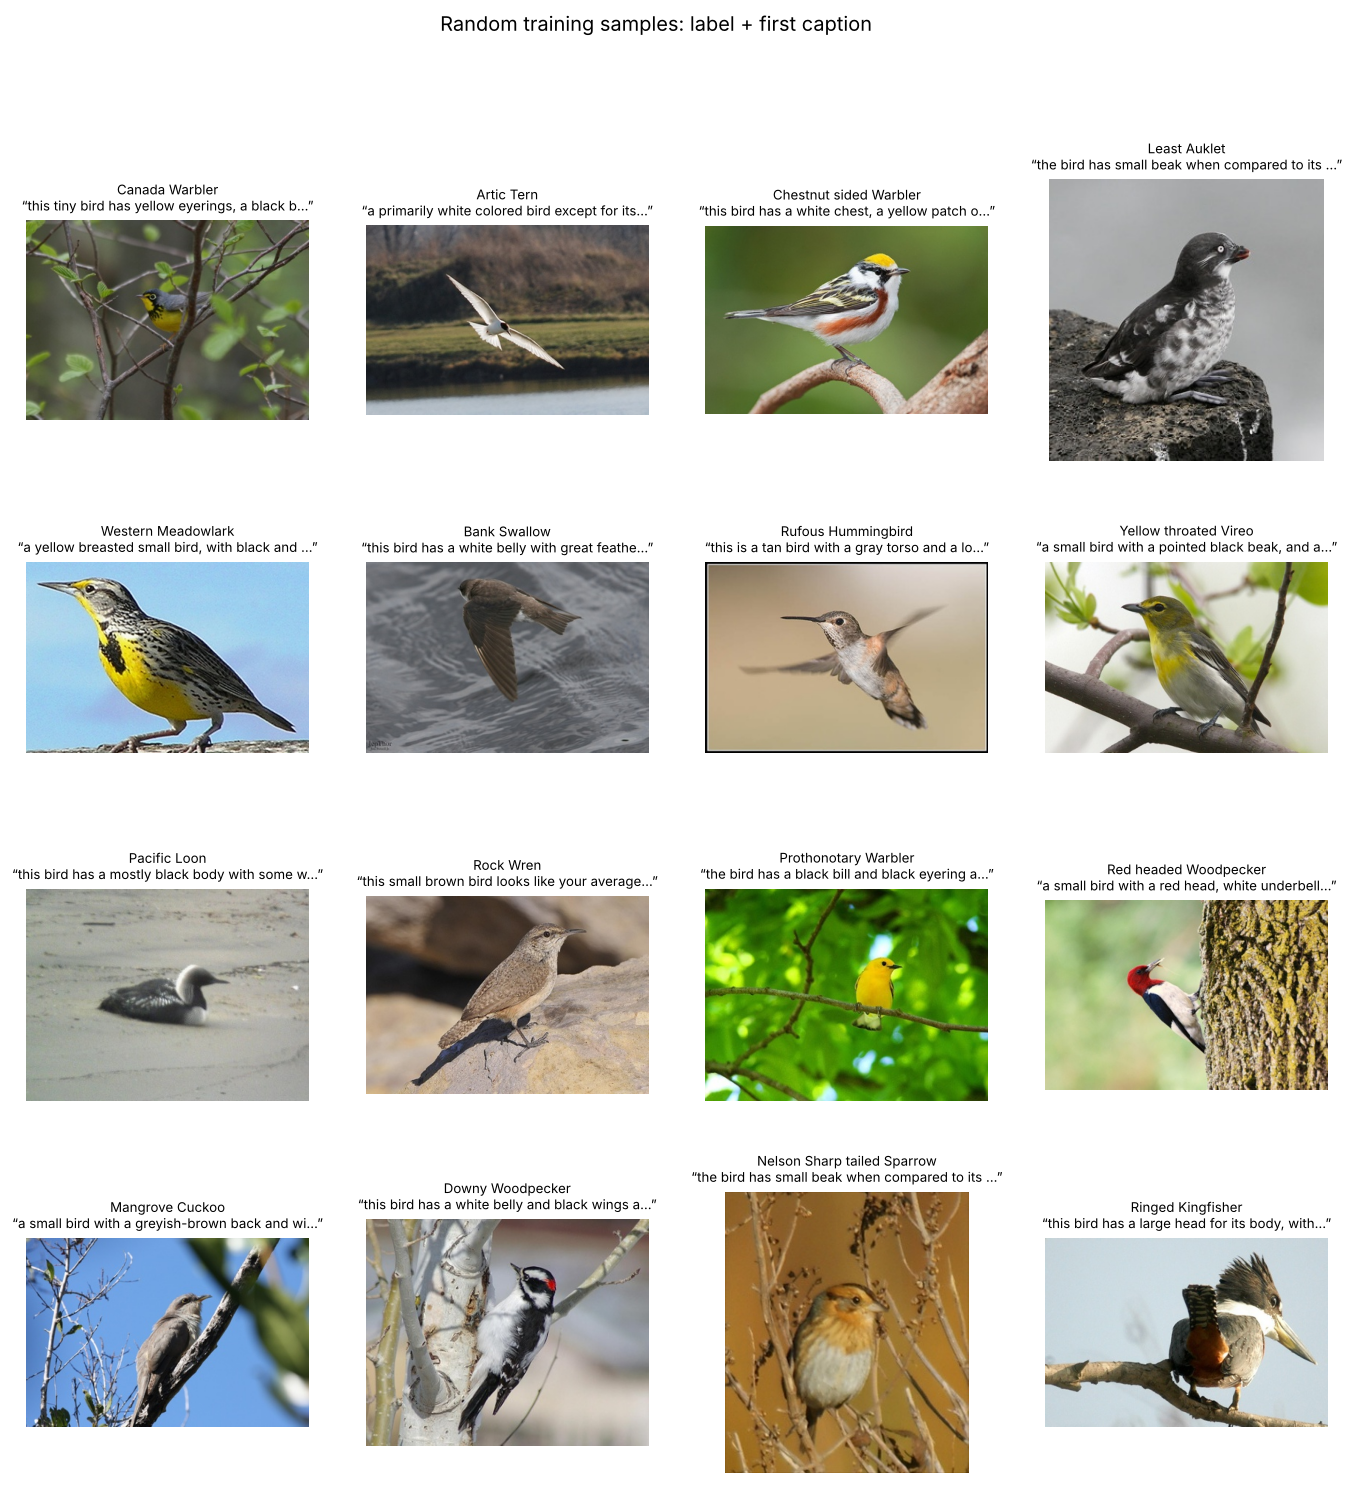
\includegraphics[width=0.78\linewidth]{figs/01_sample_grid.png}
\caption{Random training images with their label and the first of their ten captions.}
\end{figure}

\subsection{Class distribution}
The training split is almost perfectly balanced (26--27 images per class), but the \textbf{test split is
not}: most classes have 30 images, while a few have far fewer (Least Auklet 11, Crested Auklet 14, Spotted
Catbird 15; max/min ratio 2.7). Plain accuracy is therefore dominated by the large classes, which is why
we also report \textbf{macro}-averaged precision, recall and F1 (Section~\ref{sec:eval}).

\begin{figure}[H]\centering
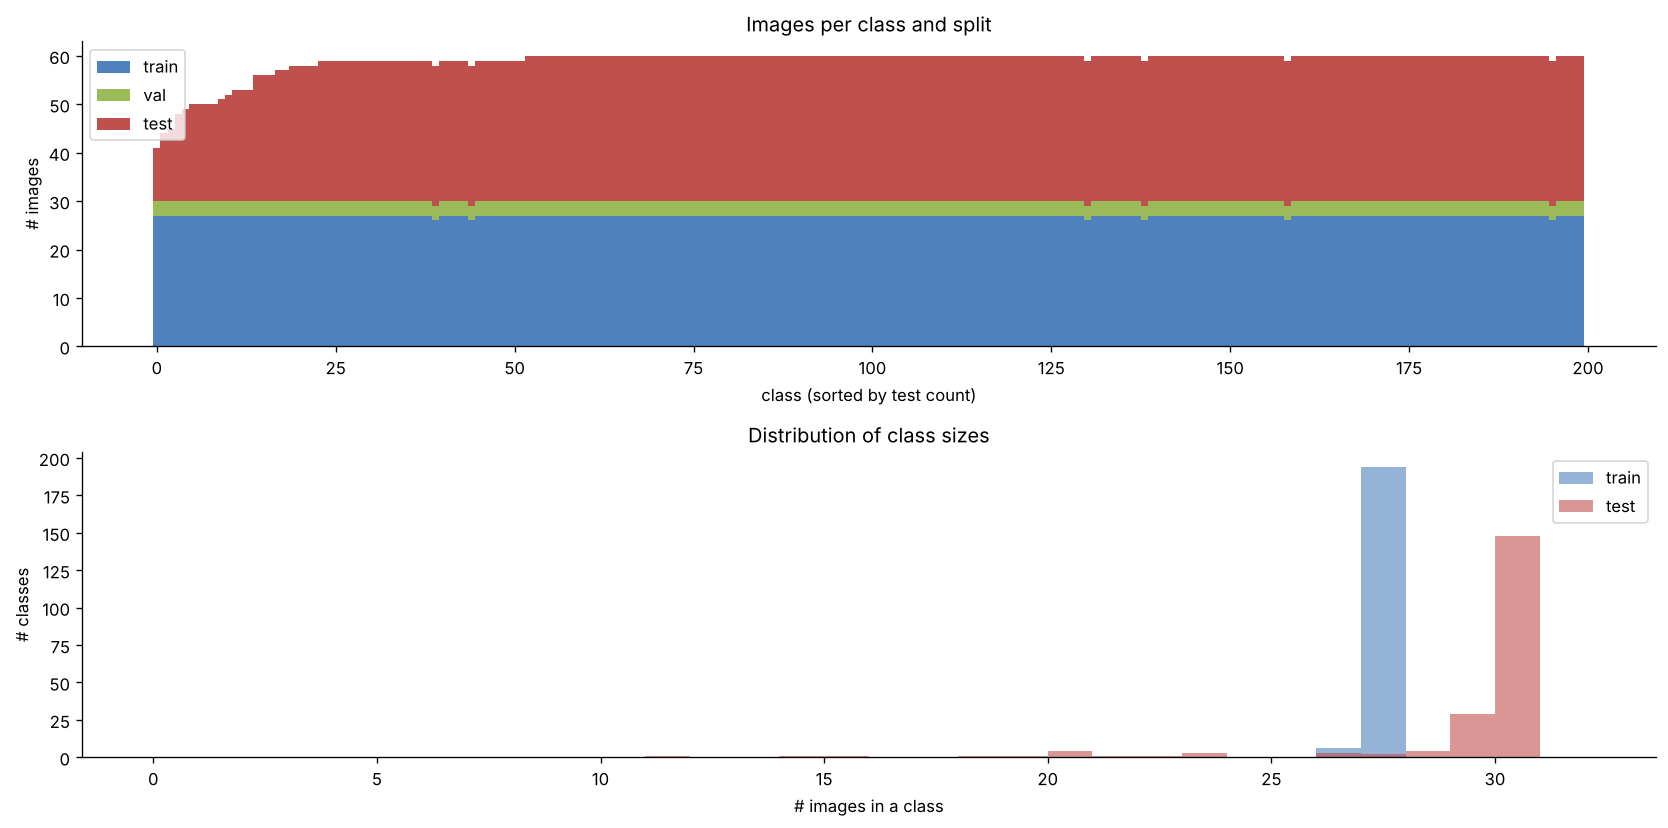
\includegraphics[width=0.9\linewidth]{figs/02_class_distribution.png}
\caption{Top: images per class and split (sorted by test count). Bottom: distribution of class sizes.}
\end{figure}

\begin{figure}[H]\centering
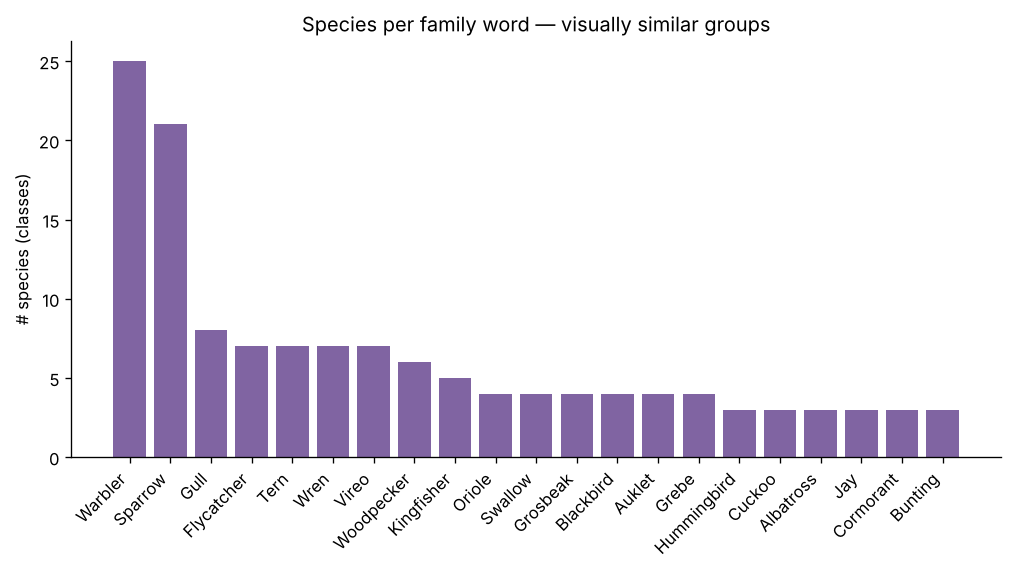
\includegraphics[width=0.7\linewidth]{figs/03_family_groups.png}
\caption{Number of species per family word. Large groups of visually similar species are the core
difficulty of fine-grained classification.}\label{fig:family}
\end{figure}

\subsection{Image sizes and quality}
Images have 1,152 distinct sizes; the median is $500\times375$ (aspect ratio 1.33, range 0.38--3.60).
148 images have a shorter side below 224\,px and are slightly upsampled at training time. Brightness,
contrast, colourfulness and sharpness distributions of train and test overlap closely
(Fig.~\ref{fig:stats}), so there is no visible domain shift between the splits.
\textbf{Preprocessing decision:} every image is resized \emph{once} (shorter side 256\,px) and cached as
JPEG. Decoding full-size images every epoch was the main bottleneck on small GPUs; the cache made each
epoch several times faster. Models then use $224\times224$ crops.

\begin{figure}[H]\centering
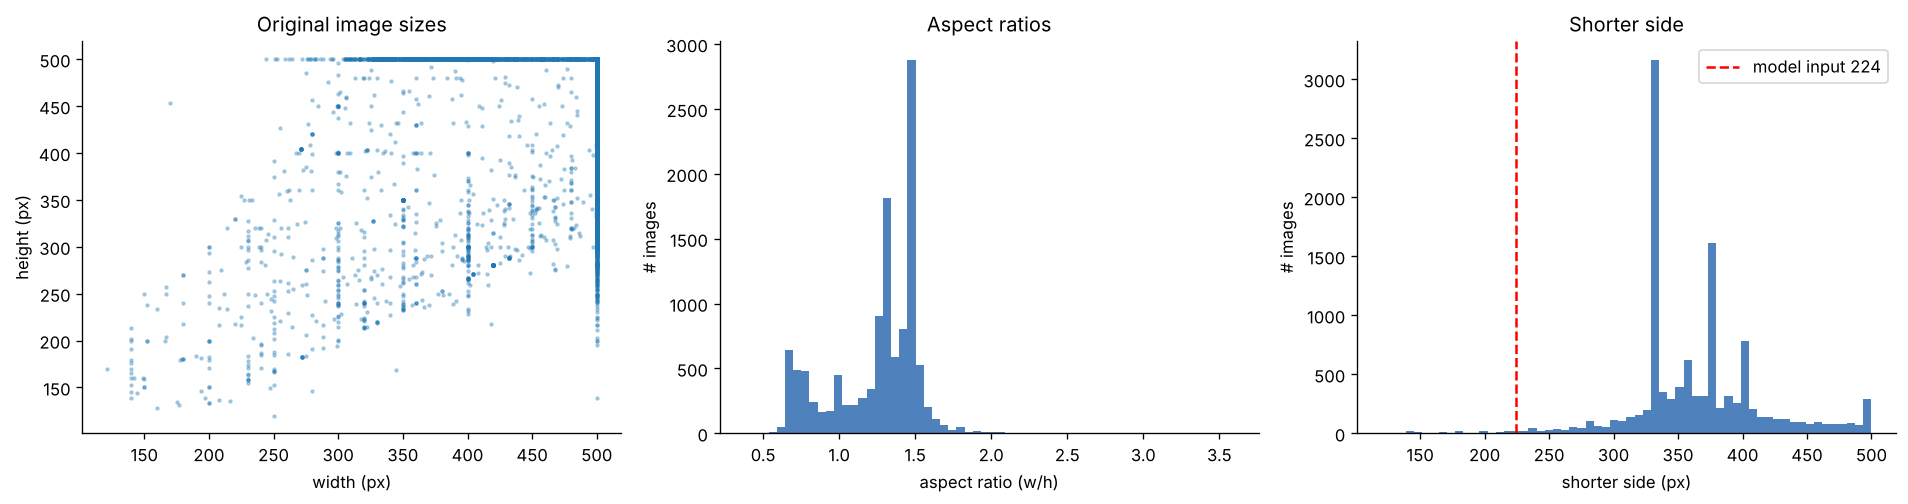
\includegraphics[width=\linewidth]{figs/04_image_sizes.png}
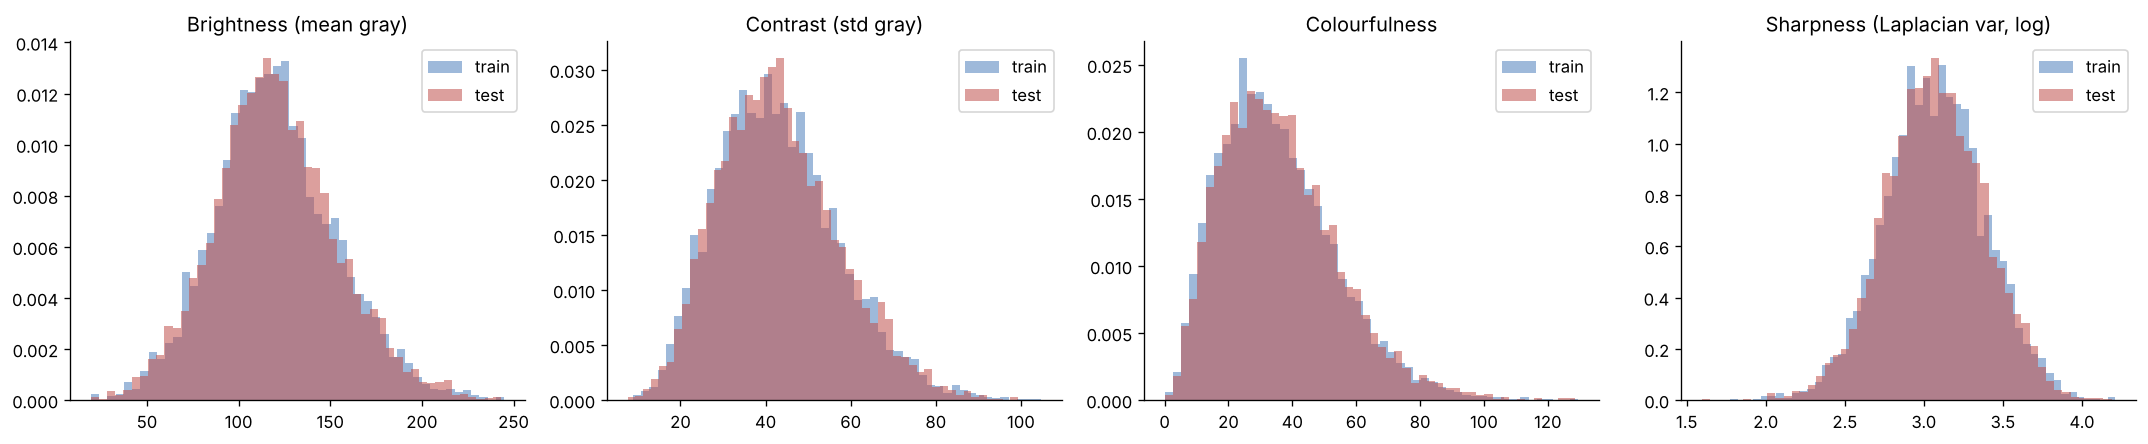
\includegraphics[width=\linewidth]{figs/05_image_statistics.png}
\caption{Image sizes (top) and per-image statistics of train vs.\ test (bottom).}\label{fig:stats}
\end{figure}

\textbf{Grayscale images.} 8 images (4 train, 4 test) are stored in grayscale mode. They are kept
for classification (converted to 3 channels), but they have no colour target and are flagged
(\texttt{is\_grayscale}) so that they are excluded from colorization in Milestone~2.

\begin{figure}[H]\centering
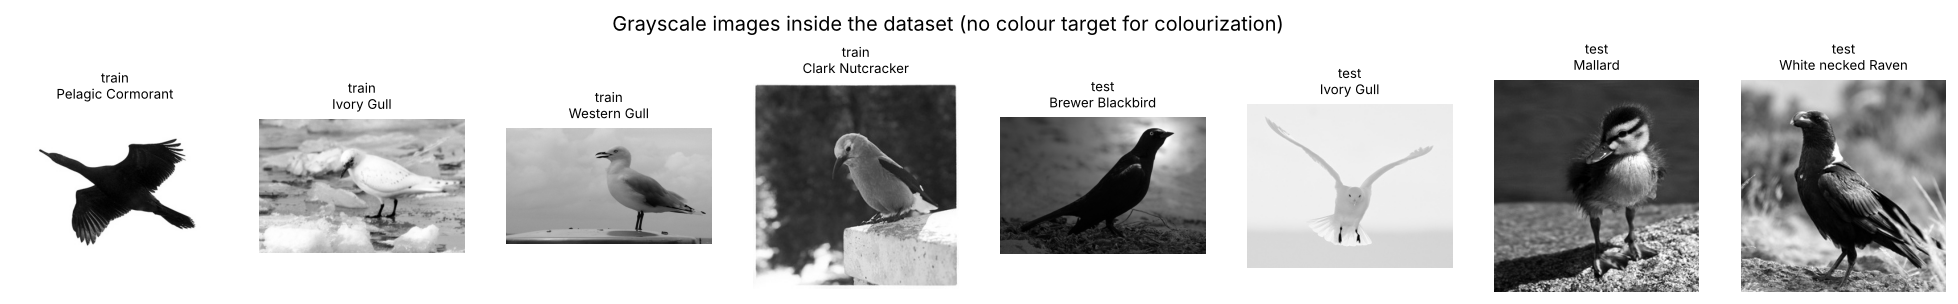
\includegraphics[width=\linewidth]{figs/08_grayscale_images.png}
\caption{The eight grayscale images in the dataset.}
\end{figure}

\subsection{Duplicates and leakage}\label{sec:dups}
Exact pixel hashing found one duplicated training image. To find re-encoded or resized copies we computed a
64-bit perceptual hash (pHash) of every image and compared all $\approx$69 million pairs. Of the 12 pairs
within Hamming distance 4, \textbf{8 pairs at distance $\le 2$ are the same photograph} (red in
Fig.~\ref{fig:dups}); the pairs at distance 3--4 are different photographs with a similar composition.
The 8 duplicates include:
\begin{itemize}
\item \textbf{2 validation$\leftrightarrow$test leaks} (Bronzed Cowbird, Prothonotary Warbler): the same image
in both splits would inflate validation accuracy;
\item 2 duplicates inside the training set (Pigeon Guillemot, Swainson Warbler);
\item \textbf{1 label conflict}: the same photograph is labelled \emph{Chuck-will's-widow} and
\emph{Whip-poor-will} (both in test) --- a sign of annotation noise between two very similar nightjars;
\item 3 same-class duplicates inside the test set.
\end{itemize}
\textbf{Cleaning decision:} the 4 train/val copies are dropped automatically by \texttt{prepare}; the
official test set is never modified (so published numbers stay comparable), and its duplicates are only
reported.

\begin{figure}[H]\centering
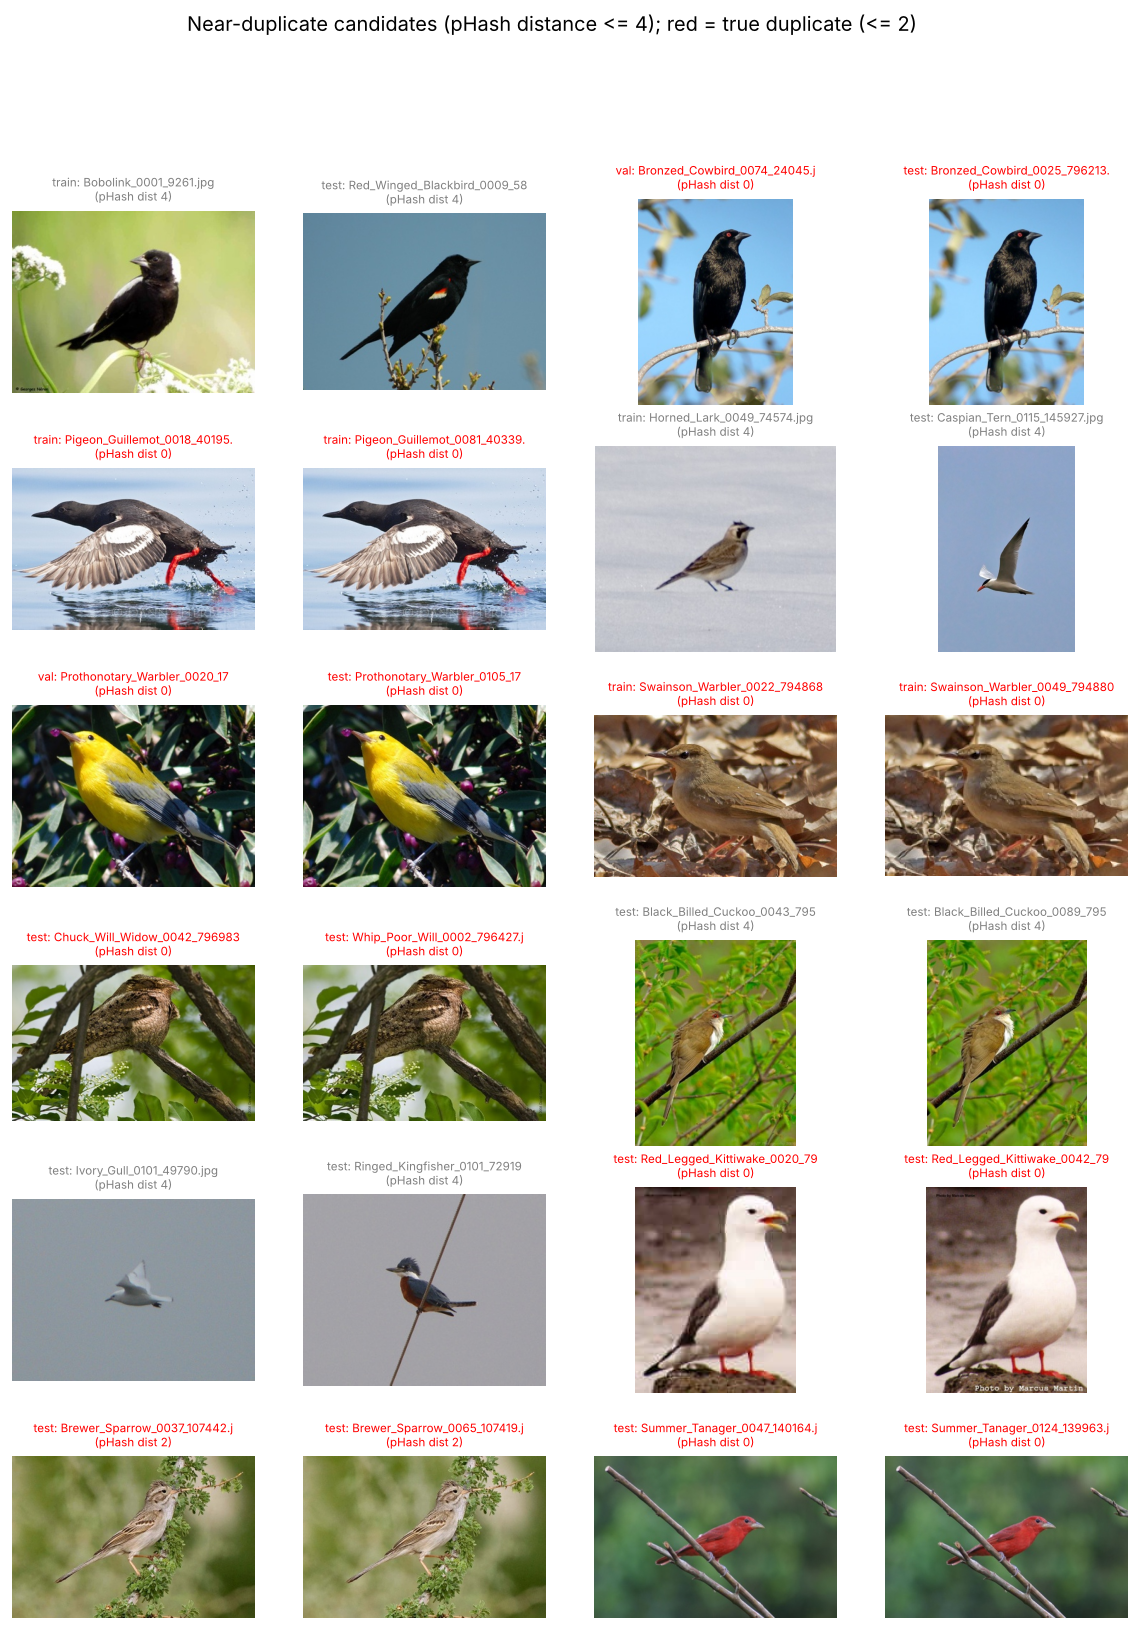
\includegraphics[width=0.85\linewidth]{figs/09_near_duplicates.png}
\caption{Duplicate candidates by perceptual hash. Red titles: true duplicates (distance $\le 2$).}\label{fig:dups}
\end{figure}

\subsection{Captions: analysis and cleaning}
The \texttt{description} field is one string per image that holds the ten captions separated by
\verb|\n| (always 11 lines: ten captions and a trailing empty line). Our analysis found:
\begin{itemize}
\item \textbf{Encoding corruption:} 1,700 Unicode replacement characters (U+FFFD), almost always in
pairs, standing in for spaces (``this\textcolor{red}{\textbf{??}}bird\textcolor{red}{\textbf{??}}has\dots'') --- most
likely non-breaking spaces that were decoded with the wrong encoding.
\item \textbf{Duplicates:} 1,306 captions repeat another caption of the same image (in 1,183 images).
\item \textbf{Templated captions:} some sentences are reused across hundreds of images, e.g.\ ``this bird
has wings that are brown and has a white belly'' appears 971 times. This matters for captioning: a decoder
can reach a decent BLEU score by producing such generic sentences.
\item \textbf{Typos and merged words:} 679 rare words are not in an English dictionary (e.g.\
``abdoment'', ``ahwite'', ``baclk'', ``ablack'', ``andthe''); they are only 0.09\% of all tokens.
\item \textbf{Uninformative captions:} 84 captions mention neither a colour nor a body part
(``a bird that lives by the ocean. it eats anything.''); conversely 98.7\% of captions contain a colour
word, confirming that colour is central to how humans describe birds.
\item \textbf{Formatting noise:} spaces before punctuation (``neck , except''), missing spaces after
commas (``breast,vent''), slashes and stray symbols.
\end{itemize}

\textbf{Cleaning pipeline} (\texttt{src/data/text.py}), applied to every line: (1) Unicode NFKC
normalisation and lower-casing; (2) replace every character outside \texttt{[a-z0-9 ,.'-]} --- including
U+FFFD --- by a space; (3) fix spacing around commas and periods; (4) collapse whitespace; (5) drop empty
lines and exact duplicates within an image, keeping order. The result is \textbf{116,574 captions}: 10 per
image for 10,605 images, 9 for 1,064, 8 for 115 and 7 for 4.
Typos are deliberately \emph{not} auto-corrected: automatic spell-checkers mis-correct domain words
(e.g.\ ``tarsus'', ``rectrices''); instead the vocabulary frequency cut-off (below) maps rare misspellings
to \texttt{<unk>}.

\textbf{Statistics.} Captions have 15.3 words on average (median 14, 95th percentile 24, 99th percentile 32,
max 66). The train+val vocabulary has 4,078 words, of which 1,872 appear only once. A minimum frequency of
5 keeps 1,243 words yet covers 99.5\% of all tokens (Fig.~\ref{fig:caps}); we will use this cut-off and a
maximum length of $\approx$32 tokens for the Milestone-2 caption decoder.

\begin{figure}[H]\centering
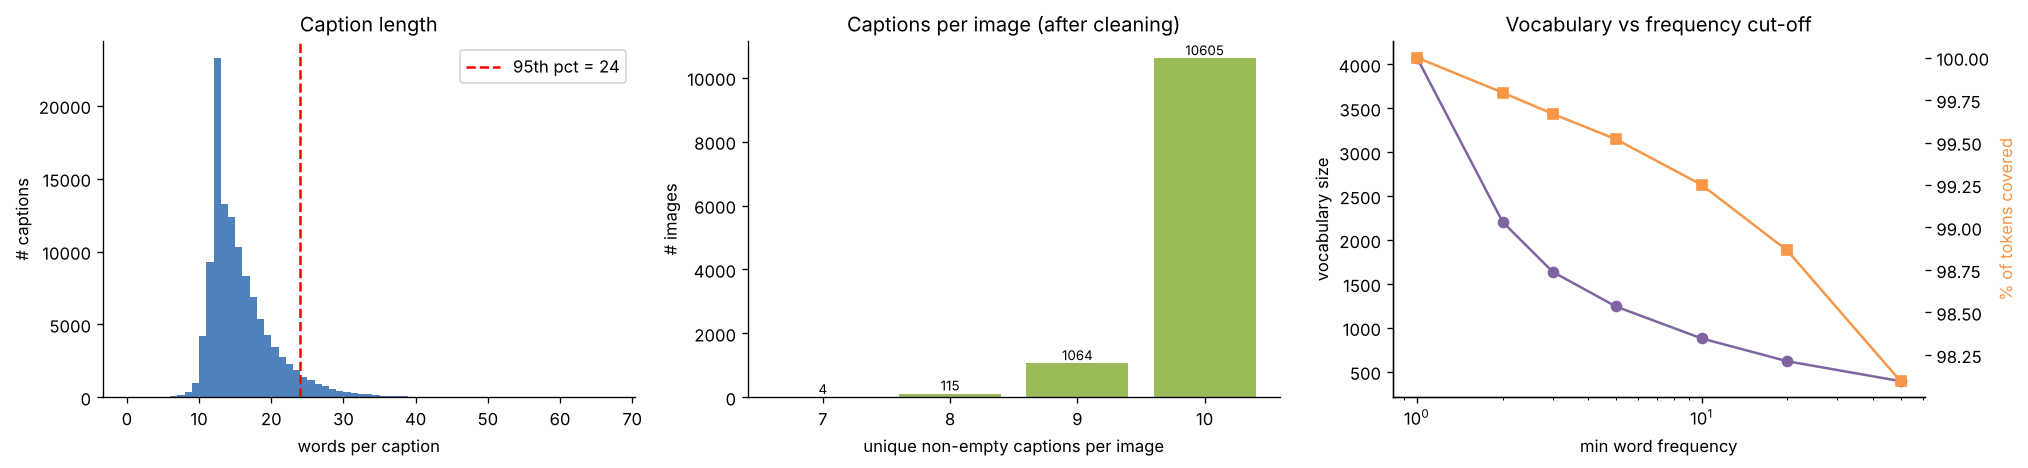
\includegraphics[width=\linewidth]{figs/10_caption_lengths_vocab.png}
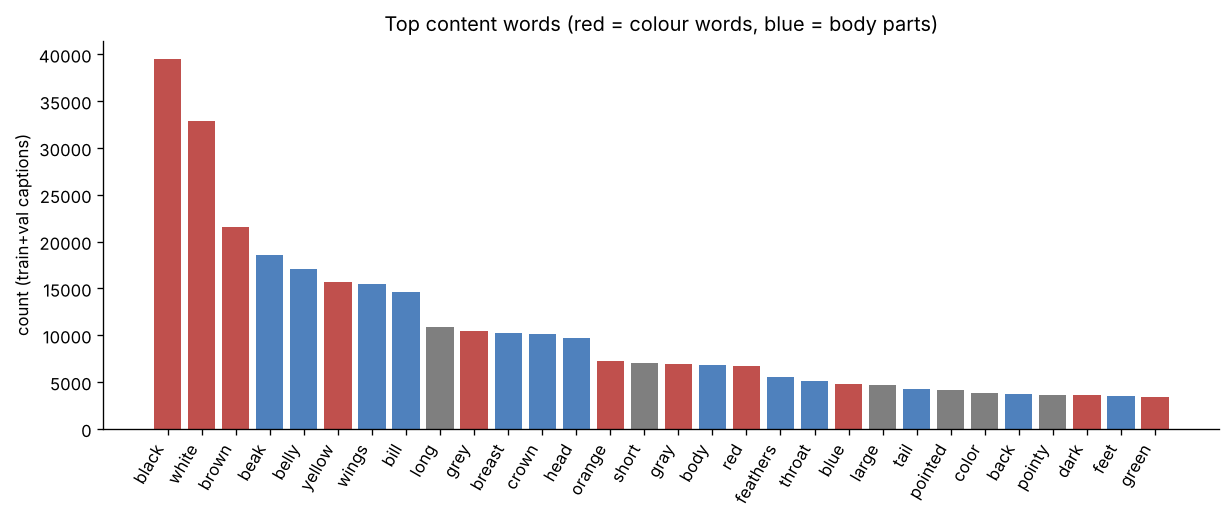
\includegraphics[width=0.85\linewidth]{figs/11_top_words.png}
\caption{Caption length, captions per image after cleaning, vocabulary size vs.\ frequency cut-off, and the most
frequent content words (red: colour words, blue: body parts).}\label{fig:caps}
\end{figure}

\subsection{Augmentation strategy}
Augmentation targets the real nuisance factors of CUB: the bird's scale and position in the frame
(RandomResizedCrop), left/right pose (horizontal flip), small camera tilt (rotation $\pm15^\circ$),
lighting (brightness/contrast $\pm20\%$, saturation $\pm10\%$) and partial occlusion by branches
(RandomErasing, $p=0.25$). \textbf{We never use hue jitter or random grayscale}: colour is one of the
most discriminative cues between species (e.g.\ Scarlet vs.\ Summer Tanager), so changing it would
create training images whose label is wrong. Three levels were implemented (Fig.~\ref{fig:aug}); the
\emph{strong} level sometimes crops the bird out of the image entirely (row 3, first sample), so
\emph{standard} is the default and \emph{light} is used for the linear probe, which has few trainable parameters.

\begin{figure}[H]\centering
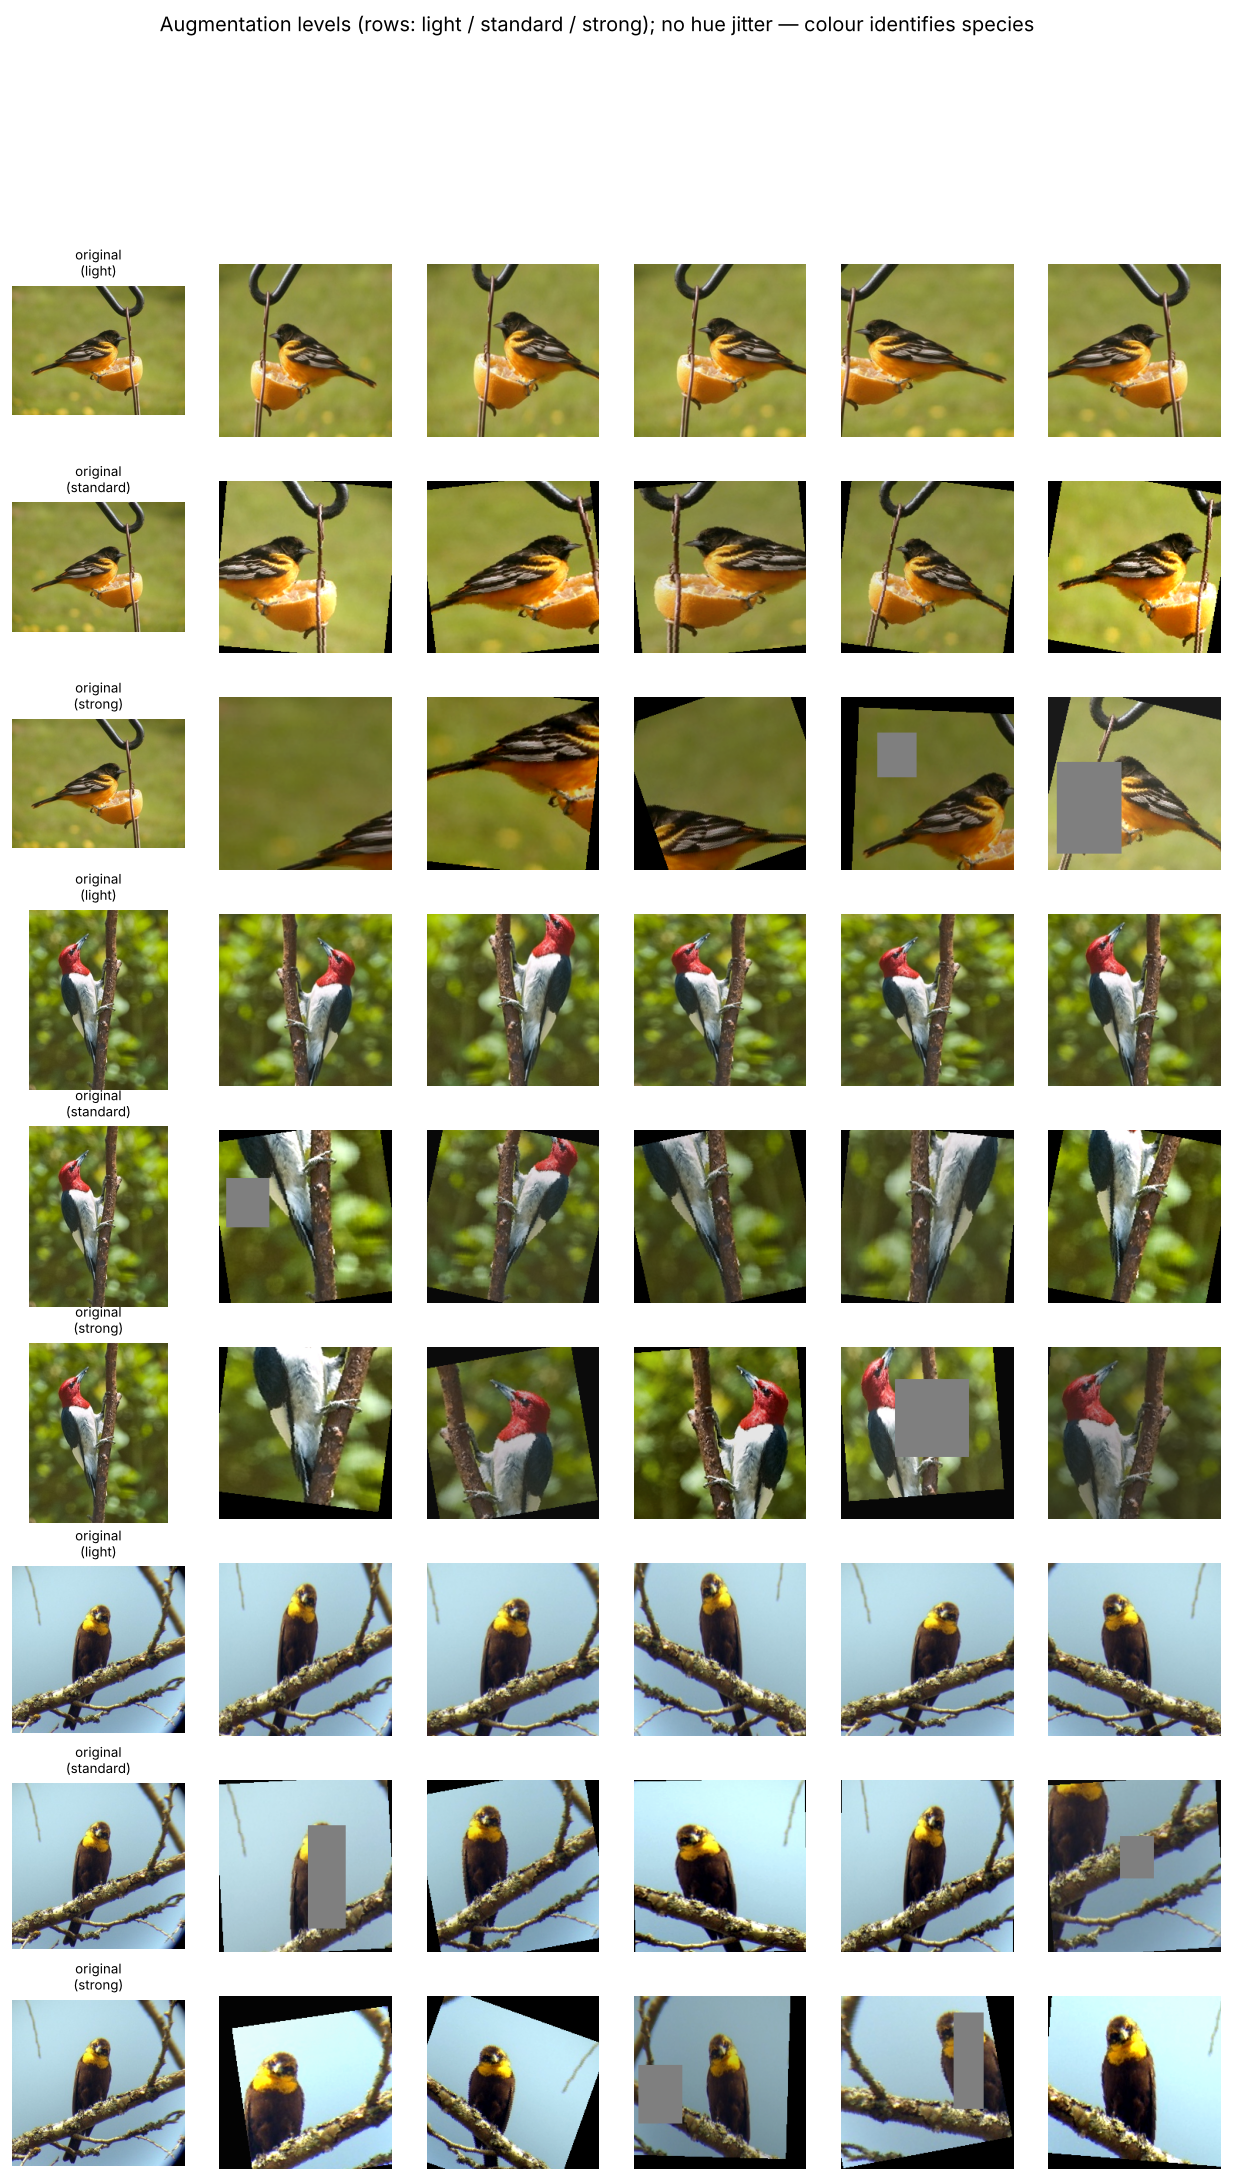
\includegraphics[width=0.72\linewidth]{figs/12_augmentation_examples.png}
\caption{Light / standard / strong augmentation on three training images.}\label{fig:aug}
\end{figure}

\subsection{How the EDA informed modelling}
\begin{itemize}
\item Imbalanced test set $\Rightarrow$ report macro-F1 and balanced accuracy, not only accuracy.
\item Only $\sim$27 images per class $\Rightarrow$ strong regularisation (label smoothing, weight decay,
dropout, augmentation) and an expectation that transfer learning will dominate training from scratch.
\item Colour is discriminative $\Rightarrow$ no hue/grayscale augmentation.
\item Small, fine details $\Rightarrow$ higher resolution would help; we use 224\,px for GPU budget reasons and
discuss this in Section~\ref{sec:fail}.
\item Duplicates and label conflict $\Rightarrow$ leak-free validation, and an explanation for one of the most
confused class pairs (Section~\ref{sec:eval}).
\end{itemize}

%=====================================================================
\section{Models}
%=====================================================================
All encoders implement one interface (\texttt{BaseEncoder} in \texttt{src/models/encoders.py}):
\texttt{forward\_features(x)} returns four feature maps at strides 4, 8, 16 and 32 (56, 28, 14 and
$7\times7$ for a 224\,px input), together with their channel counts and the layer used by Grad-CAM. Encoders are
created through a registry, so any encoder can be selected from the config without touching the training
code. The multi-scale output is designed for Milestone~2: the colorization U-Net uses all four maps as skip
connections, and the caption decoder attends over the last $7\times7$ grid. The classifier is
\emph{encoder $\rightarrow$ global average pooling $\rightarrow$ dropout $\rightarrow$ linear layer (200 classes)}.

\begin{table}[H]\centering\small
\begin{tabular}{lrll}
\toprule
Encoder & Params & Initialisation & Notes\\
\midrule
Scratch CNN (ours) & 11.3M & random (Kaiming) & residual, 4 stages $64\!-\!128\!-\!256\!-\!512$, 2 blocks each\\
Scratch CNN, no skips & 11.1M & random & ablation: same CNN without residual connections\\
ResNet-50~\cite{resnet} & 23.9M & ImageNet & bottleneck residual network\\
EfficientNet-B0~\cite{effnet} & 4.3M & ImageNet & depthwise convs + squeeze-excitation, compound scaling\\
ConvNeXt-Tiny~\cite{convnext} & 28.0M & ImageNet & modernised ResNet: $7\times7$ depthwise convs, LayerNorm, GELU\\
\bottomrule
\end{tabular}
\caption{Encoders (parameter counts include the 200-class head).}
\end{table}

\textbf{Our from-scratch CNN.} Stem: $3\times3$ conv (stride 2) $\rightarrow$ $3\times3$ conv $\rightarrow$
max-pool; then four stages of two residual blocks ($3\times3$ conv--BN--ReLU--$3\times3$ conv--BN, plus an
identity or $1\times1$ projection shortcut). Every stage after the first halves the resolution and doubles the
channels. Weights use Kaiming initialisation, and the last BatchNorm of every residual branch is initialised
to zero so that each block starts as an identity mapping, which stabilises early training.

\textbf{Transfer-learning strategies.} (a) \emph{Linear probe}: the ImageNet backbone is frozen (including its
BatchNorm statistics) and only the linear head is trained. (b) \emph{Full fine-tuning}: all layers are trained,
with \emph{discriminative learning rates} --- the head uses the base LR and the pretrained backbone uses
$0.1\times$ that LR, so the useful ImageNet features are adapted gently instead of being overwritten.

%=====================================================================
\section{Experiments}
%=====================================================================
\textbf{Common setup.} AdamW, linear warm-up then cosine decay (per step), label smoothing 0.1, mixed precision
(FP16), batch size 32 (64 for the scratch CNNs), $224\times224$ inputs, ImageNet normalisation for pretrained
models and dataset statistics (mean $[0.485, 0.499, 0.432]$) for the scratch models, early stopping on
validation accuracy with the best checkpoint restored. Hardware: one NVIDIA Tesla T4 (Kaggle). One run per
configuration, seed 42.

\begin{table}[H]\centering\small
\begin{tabular}{lcccccc}
\toprule
Run & LR (head) & Weight decay & Aug. & Epochs (best) & Time & s/epoch\\
\midrule
Scratch CNN & 2e-3 & 0.05 & standard & 80 (64) & 23.8 min & 17.8\\
Scratch CNN, no skips & 2e-3 & 0.05 & standard & 40 (37) & 11.8 min & 17.7\\
ResNet-50 linear probe & 3e-3 & 1e-4 & light & 15 (11) & 5.1 min & 20.2\\
ResNet-50 fine-tune & 1e-3 & 1e-4 & standard & 30 (27) & 9.9 min & 19.7\\
ResNet-50 fine-tune, tuned & 2.09e-3 & 3.4e-5 & standard & 30 (23) & 11.7 min & 23.4\\
EfficientNet-B0 fine-tune & 1e-3 & 1e-4 & standard & 30 (29) & 10.4 min & 20.8\\
ConvNeXt-Tiny fine-tune & 1e-3 & 1e-4 & standard & 28 (20) & 13.5 min & 28.8\\
\bottomrule
\end{tabular}
\caption{Settings of every training run. Pretrained backbones use $0.1\times$ the head LR.}
\end{table}

\begin{table}[H]\centering\small
\begin{tabular}{lcccccc}
\toprule
Model & Accuracy & Top-5 & Precision & Recall & F1 & Best val acc\\
\midrule
Scratch CNN, no skips & 36.5 & 67.0 & 35.5 & 36.7 & 35.0 & 36.0\\
Scratch CNN (ours) & 52.5 & 76.7 & 53.2 & 52.5 & 52.1 & 51.7\\
ResNet-50 linear probe & 67.6 & 91.2 & 69.0 & 68.0 & 67.7 & 66.4\\
EfficientNet-B0 fine-tune & 79.8 & 94.4 & 80.3 & 80.0 & 79.8 & 79.1\\
ResNet-50 fine-tune & 82.4 & 95.2 & 82.8 & 82.5 & 82.3 & 81.6\\
ResNet-50 fine-tune, tuned & 82.4 & 95.3 & 82.8 & 82.6 & 82.3 & 81.8\\
\textbf{ConvNeXt-Tiny fine-tune} & \textbf{84.6} & \textbf{96.0} & \textbf{85.0} & \textbf{84.8} & \textbf{84.5} & \textbf{84.3}\\
\bottomrule
\end{tabular}
\caption{Test-set results (\%, official CUB test split, 5,794 images). Precision/recall/F1 are macro-averaged.}\label{tab:results}
\end{table}

\begin{figure}[H]\centering
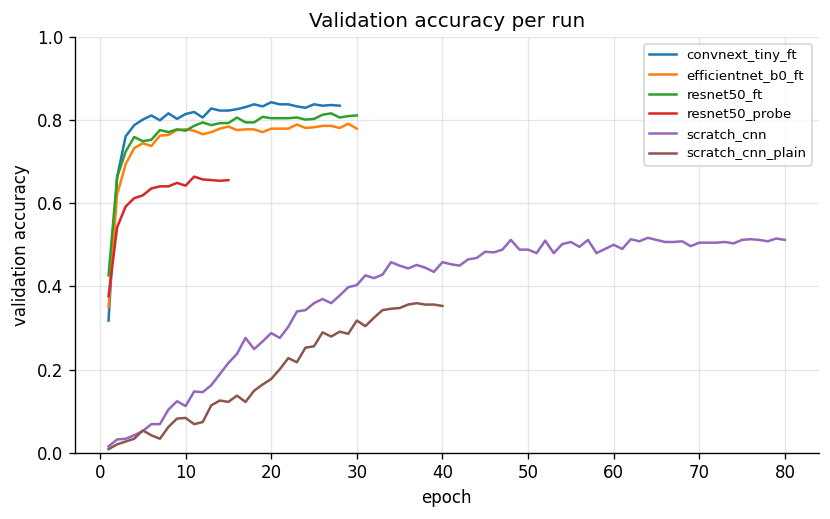
\includegraphics[width=0.75\linewidth]{figs/val_curves.png}
\caption{Validation accuracy per epoch for all runs.}\label{fig:val}
\end{figure}

\subsection{From scratch vs.\ transfer learning}
Transfer learning wins by a wide margin: the best fine-tuned model is \textbf{32 points} more accurate than our
scratch CNN, converges in 20 epochs instead of 64, and is already at $\sim$75\% validation accuracy after
3 epochs (Fig.~\ref{fig:val}). With only $\sim$27 images per class, a network trained from scratch must learn
edges, textures and bird parts from about 5,400 images; ImageNet pretraining provides these generic features for free.

The scratch CNN also shows the clearest \textbf{overfitting} (Fig.~\ref{fig:scratch}): training accuracy reaches 96\%
while validation accuracy plateaus at 51\%, and the validation loss stops improving after epoch $\sim$45 while the
training loss keeps falling. Strong regularisation (weight decay 0.05, dropout 0.3, label smoothing, RandomErasing)
reduced but could not close this gap. The pretrained models also fit the training set ($>98\%$), but their gap is
much smaller because their features generalise.

\textbf{Linear probe vs.\ fine-tuning.} Frozen ImageNet features already give 67.6\%, i.e.\ they are informative about
birds; but fine-tuning the whole backbone adds \textbf{+14.8 points}. ImageNet features are tuned to separate e.g.\
``bird vs.\ dog'', not ``California Gull vs.\ Western Gull'', so adapting the deeper layers to fine-grained cues is essential.

\textbf{Ablation: residual connections.} With the same 11M-parameter CNN, removing the skip connections lowers validation
accuracy at epoch 40 from 45.8\% to 35.3\%. Crucially the no-skip network does \emph{not} overfit --- its training accuracy
is only 44\% --- it is harder to \emph{optimise}. This is the degradation problem described by He et al.~\cite{resnet}:
residual connections give gradients a short path through the 18-layer network.

\begin{figure}[H]\centering
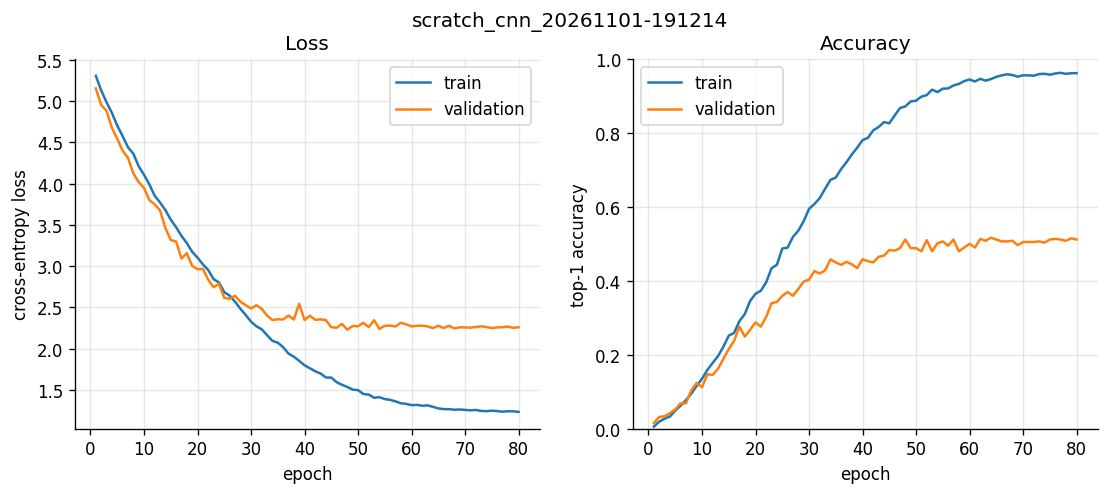
\includegraphics[width=0.49\linewidth]{figs/curves_scratch.png}
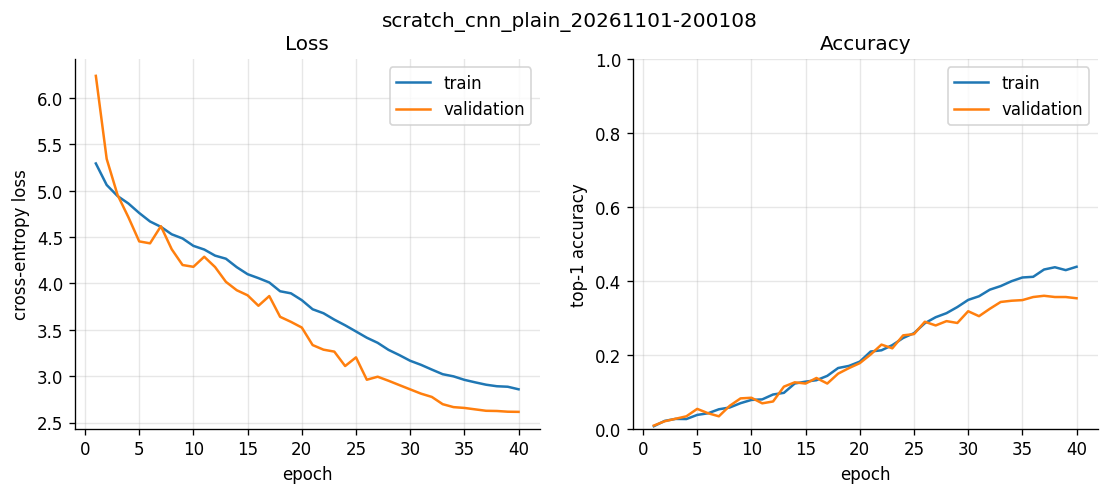
\includegraphics[width=0.49\linewidth]{figs/curves_scratch_plain.png}
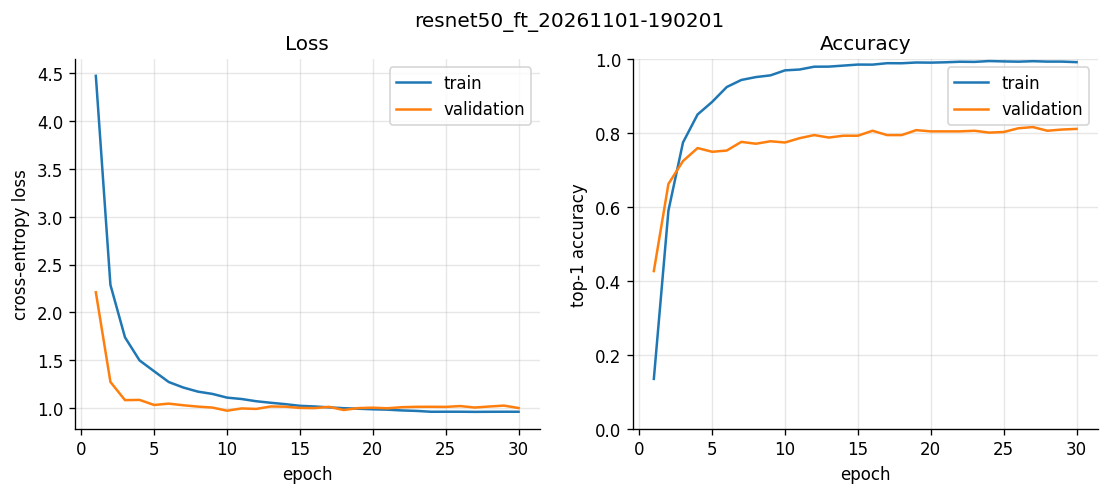
\includegraphics[width=0.49\linewidth]{figs/curves_resnet50_ft.png}
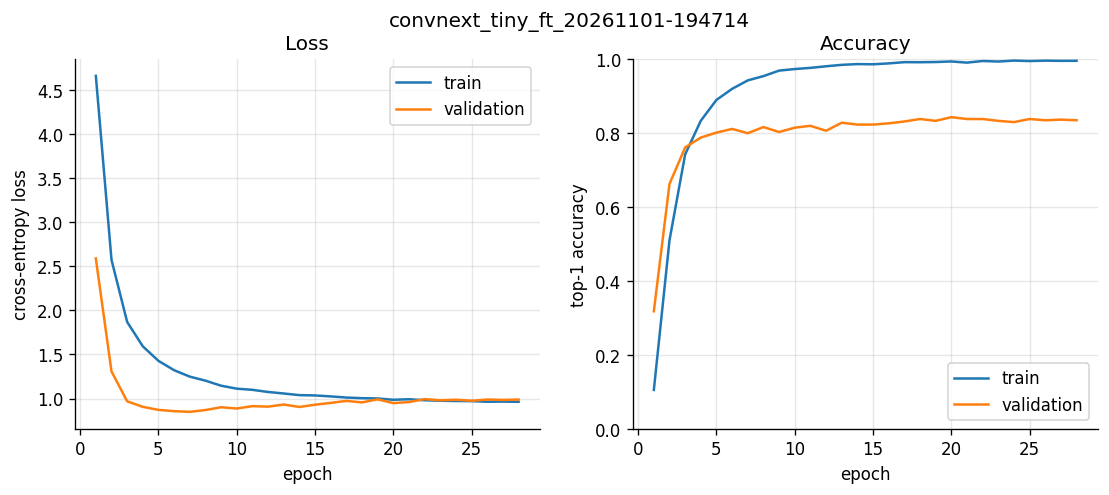
\includegraphics[width=0.49\linewidth]{figs/curves_convnext.png}
\caption{Training vs.\ validation loss and accuracy. Top: scratch CNN with and without residual connections.
Bottom: fine-tuned ResNet-50 and ConvNeXt-Tiny.}\label{fig:scratch}
\end{figure}

\subsection{Architecture comparison}
Among pretrained backbones, ConvNeXt-Tiny is best (84.6\%), ResNet-50 second (82.4\%) and EfficientNet-B0 third
(79.8\%), which matches their ordering on ImageNet and the finding of Kornblith et al.~\cite{kornblith} that better
ImageNet architectures transfer better. EfficientNet-B0 is the most parameter-efficient (79.8\% with 4.3M parameters,
$6.6\times$ fewer than ConvNeXt), while ConvNeXt costs about 45\% more time per epoch than ResNet-50.

\begin{figure}[H]\centering
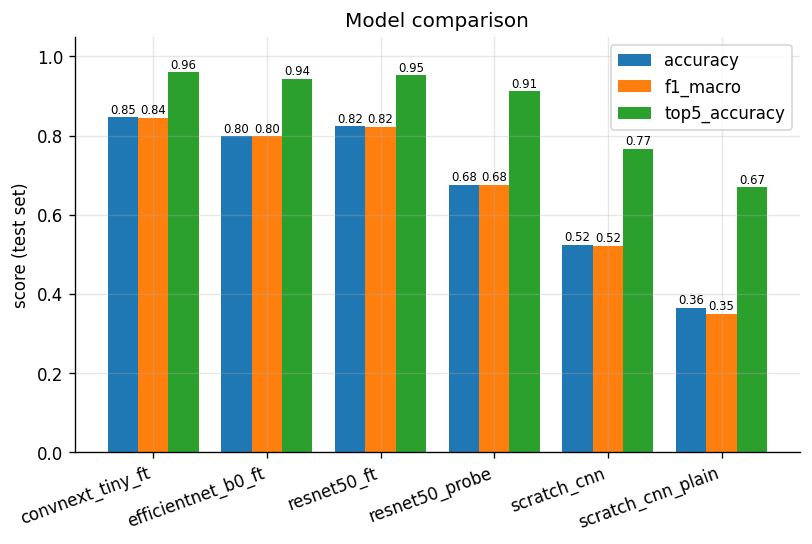
\includegraphics[width=0.8\linewidth]{figs/comparison.png}
\caption{Test accuracy, macro-F1 and top-5 accuracy of all models.}
\end{figure}

%=====================================================================
\section{Hyper-parameter tuning}\label{sec:tuning}
%=====================================================================
\textbf{Setup.} We tuned the two hyper-parameters with the largest expected effect for fine-tuning, the
\textbf{learning rate} (head LR; backbone $=0.1\times$) and \textbf{weight decay}, on ResNet-50 full fine-tuning.
Each trial is a short 8-epoch run (enough to rank configurations); selection uses only the validation set.
\begin{itemize}
\item \textbf{Grid search:} LR $\in\{3\!\times\!10^{-4}, 10^{-3}, 3\!\times\!10^{-3}\}$ $\times$ WD $\in\{10^{-5}, 10^{-4}, 10^{-3}\}$ = 9 trials.
\item \textbf{Random search~\cite{bergstra}:} 9 trials (same budget), LR $\sim$ log-uniform$[2\!\times\!10^{-4}, 5\!\times\!10^{-3}]$,
WD $\sim$ log-uniform$[10^{-5}, 10^{-2}]$, i.e.\ the same ranges.
\end{itemize}

\begin{table}[H]\centering\small
\begin{tabular}{lcccc}
\toprule
Method & Trials & Best val acc & Total time & Best found at\\
\midrule
Grid & 9 & 79.3\% (LR 3e-3, WD 1e-4) & 25.3 min & trial 8\\
Random & 9 & \textbf{80.4\%} (LR 2.09e-3, WD 3.4e-5) & 24.3 min & trial 8\\
\bottomrule
\end{tabular}
\caption{Comparison of tuning methods with the same budget.}
\end{table}

\begin{figure}[H]\centering
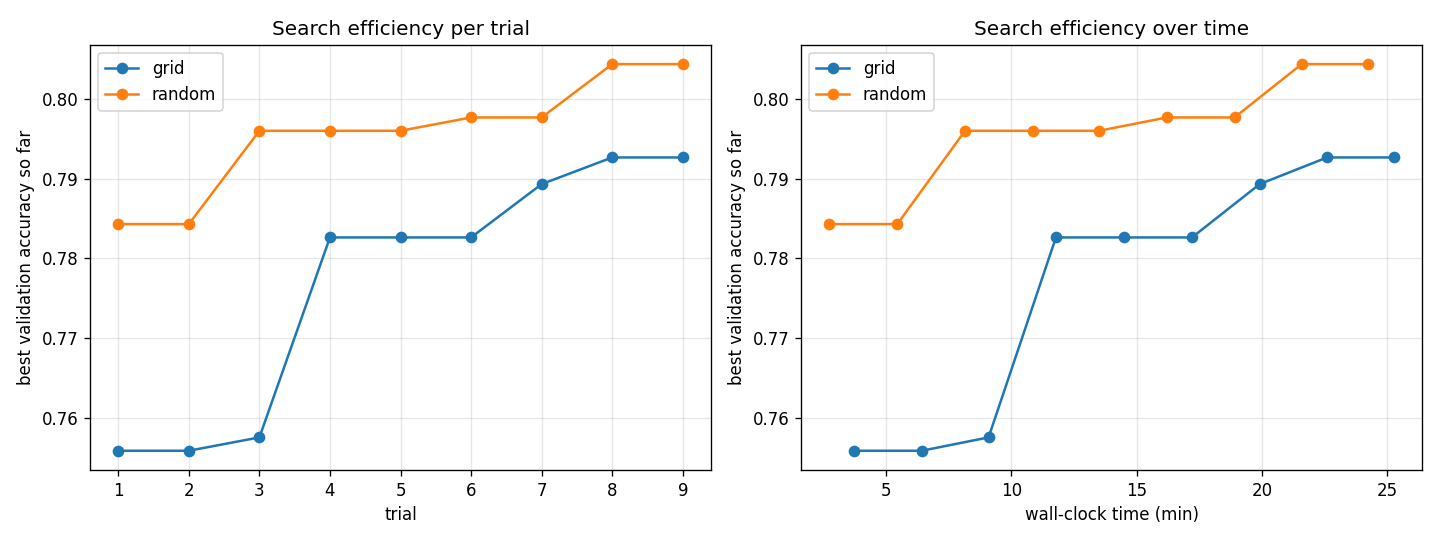
\includegraphics[width=\linewidth]{figs/tuning_progress.png}
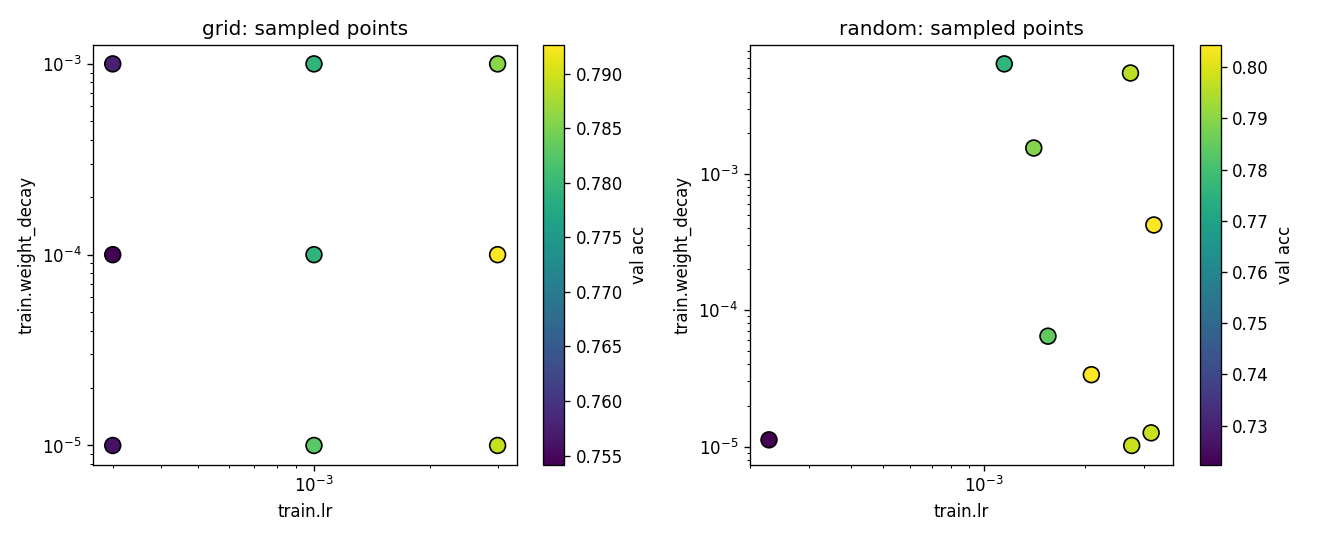
\includegraphics[width=0.9\linewidth]{figs/tuning_samples.png}
\caption{Top: best validation accuracy so far vs.\ trial number and wall-clock time. Bottom: where each method sampled
(colour = validation accuracy).}
\end{figure}

\textbf{Findings.}
\begin{enumerate}
\item \textbf{Learning rate dominates; weight decay barely matters.} In the grid, the mean accuracy per LR row is
75.6\%, 78.0\% and 78.9\% for LR $3\!\times\!10^{-4}$, $10^{-3}$ and $3\!\times\!10^{-3}$, while changing WD by $100\times$
moves accuracy by less than 0.7 points.
\item \textbf{Random search was better with the same budget} (80.4\% vs.\ 79.3\%, and ahead after every trial). Grid
search spends three trials on each LR value; random search tries 9 different LR values, which is more useful when only
one of the two dimensions is important~\cite{bergstra}. The grid's best LR is also on the edge of its range, a sign the
grid was too narrow; random search covered more of the LR axis.
\item \textbf{Caveat: noise.} With 598 validation images one image is 0.17\%, and the standard error of an accuracy near
80\% is about $\sqrt{0.8\cdot0.2/598}\approx1.6\%$. Differences of $\sim$1 point between trials are within noise.
\end{enumerate}

\textbf{Baseline vs.\ tuned model.} Retraining ResNet-50 for the full 30 epochs with the best random-search
configuration gave 82.40\% test accuracy vs.\ 82.38\% for the default configuration --- \textbf{no meaningful
improvement}. The short 8-epoch proxy rewards hyper-parameters that converge \emph{fast} (a higher LR), but with a full
cosine schedule the default LR catches up. We report this honestly as a limitation of low-fidelity tuning: the proxy
should be closer to the real schedule (e.g.\ 15--20 epochs) or combined with a multi-fidelity method such as Hyperband.

%=====================================================================
\section{Experiment tracking}
%=====================================================================
Every run is logged with Weights \& Biases~\cite{wandb} through a small \texttt{Tracker} interface
(\texttt{src/tracking/trackers.py}); a local tracker additionally writes \texttt{config.yaml},
\texttt{history.jsonl}, \texttt{summary.json} and the plots to each run folder, so all figures can be regenerated
offline. For each run we log: the full configuration (all hyper-parameters, encoder, augmentation, seed), per-epoch
train/validation loss and accuracy, validation macro-F1 and top-5, learning rate and epoch time, the final test metrics,
parameter counts, the device, and the path of the best checkpoint. Tuning trials are grouped
(\texttt{tune-grid-*}, \texttt{tune-random-*}) and tagged, so the two searches can be compared side by side.
In total Milestone~1 contains 53 runs: 7 baseline training runs, 18 tuning-v1 trials, 16 improvement runs, 8 tuning-v2 trials
and 4 final runs.

\begin{figure}[H]\centering
\shot{wandb_runs.png}{Screenshot: W\&B project page --- run table with all runs, their configs and test accuracy}
\caption{W\&B: all runs of Milestone 1.}
\end{figure}
\begin{figure}[H]\centering
\shot{wandb_charts.png}{Screenshot: W\&B charts --- val\_acc and train/val loss of the 7 training runs overlaid}
\caption{W\&B: learning curves of the training runs.}
\end{figure}
\begin{figure}[H]\centering
\shot{wandb_tuning.png}{Screenshot: W\&B tuning group --- parallel-coordinates plot of lr, weight\_decay and val\_acc}
\caption{W\&B: hyper-parameter search trials.}
\end{figure}

%=====================================================================
\section{Evaluation}\label{sec:eval}
%=====================================================================
\textbf{Metrics.}
\begin{itemize}
\item \textbf{Accuracy}: fraction of test images whose top-1 prediction is correct. Simple, but dominated by the larger
classes of the imbalanced test set.
\item \textbf{Top-5 accuracy}: the true class is among the five most probable. In fine-grained tasks the top-2/3 are often
sibling species, so top-5 shows whether the model at least narrows the answer to the right group.
\item \textbf{Macro precision / recall / F1}: computed per class and averaged with equal weight, so the small classes
(e.g.\ Least Auklet, 11 images) count as much as the large ones. Precision: of the images predicted as class $c$, how many are $c$;
recall: of the images of class $c$, how many were found; F1: their harmonic mean.
\item \textbf{Balanced accuracy}: mean per-class recall.
\item \textbf{Confusion matrix} and the list of the most confused class pairs.
\end{itemize}

\textbf{Interpretation.} For every model, macro-F1 is within 0.5 points of accuracy (Table~\ref{tab:results}), so the test
imbalance does not hide a failure on small classes. ConvNeXt's top-5 accuracy of 96.0\% means that for 96\% of images the
correct species is among five candidates --- the remaining errors are mostly between siblings. Its per-class accuracy ranges
from 100\% (e.g.\ the woodpeckers with distinctive patterns) down to 23\% (California Gull, Common Tern).

\begin{figure}[H]\centering
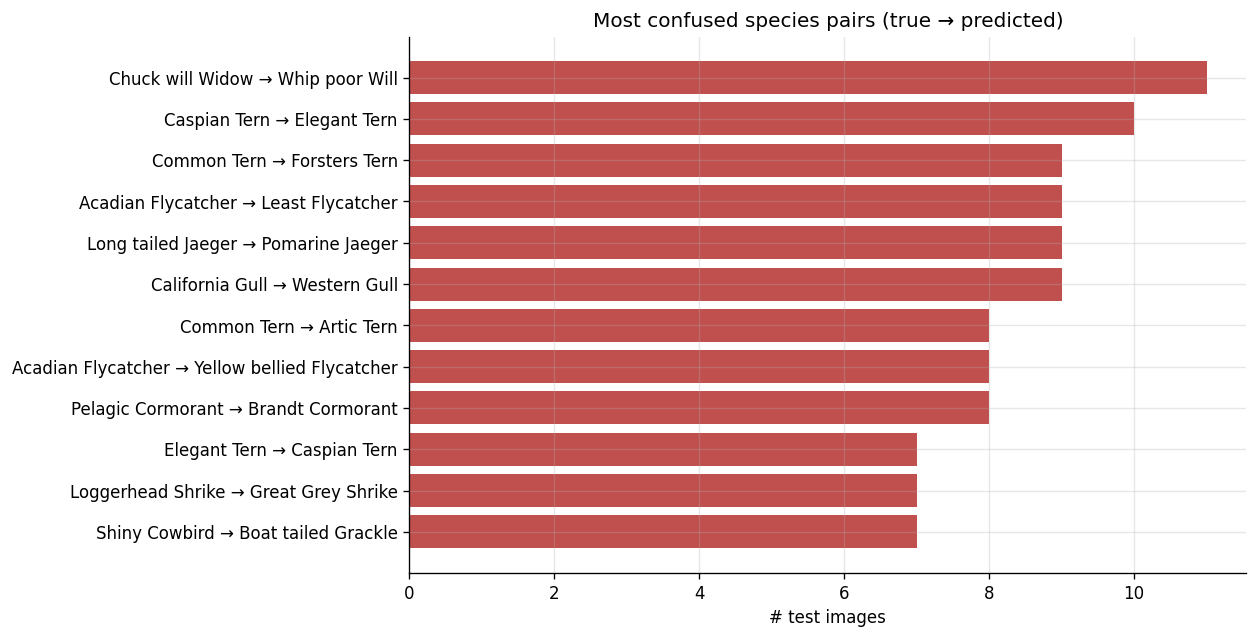
\includegraphics[width=0.75\linewidth]{figs/confused_convnext.png}
\caption{Most confused (true $\rightarrow$ predicted) pairs of ConvNeXt-Tiny on the test set.}\label{fig:conf}
\end{figure}

The most confused pairs (Fig.~\ref{fig:conf}) are exactly the hard fine-grained cases: terns (Caspian/Elegant,
Common/Forster's/Arctic), gulls (California/Western), \emph{Empidonax} flycatchers (Acadian/Least/Yellow-bellied) and jaegers ---
species that birders separate by size, voice or subtle bill and wing-tip details that are hard to see at 224\,px.
The top pair, \textbf{Chuck-will's-widow $\rightarrow$ Whip-poor-will} (11 of 26 test images), is the same pair for which the EDA
found an identical photograph labelled as both species --- evidence that the labels of these two nightjars are themselves noisy.

%=====================================================================
\section{Explainability (Grad-CAM)}
%=====================================================================
We implemented Grad-CAM~\cite{gradcam} (\texttt{src/visualization/gradcam.py}) with forward/backward hooks on the last
stage of each encoder. For the target class $c$, the weight of channel $k$ is the spatial mean of
$\partial y^c / \partial A^k$, and the map is $\mathrm{ReLU}(\sum_k \alpha_k^c A^k)$, upsampled to the image size. The same
test images are shown for the scratch CNN, ResNet-50 and ConvNeXt; images are selected from the scratch model's predictions
(6 random correct ones and its 6 most confident mistakes).

\begin{figure}[H]\centering
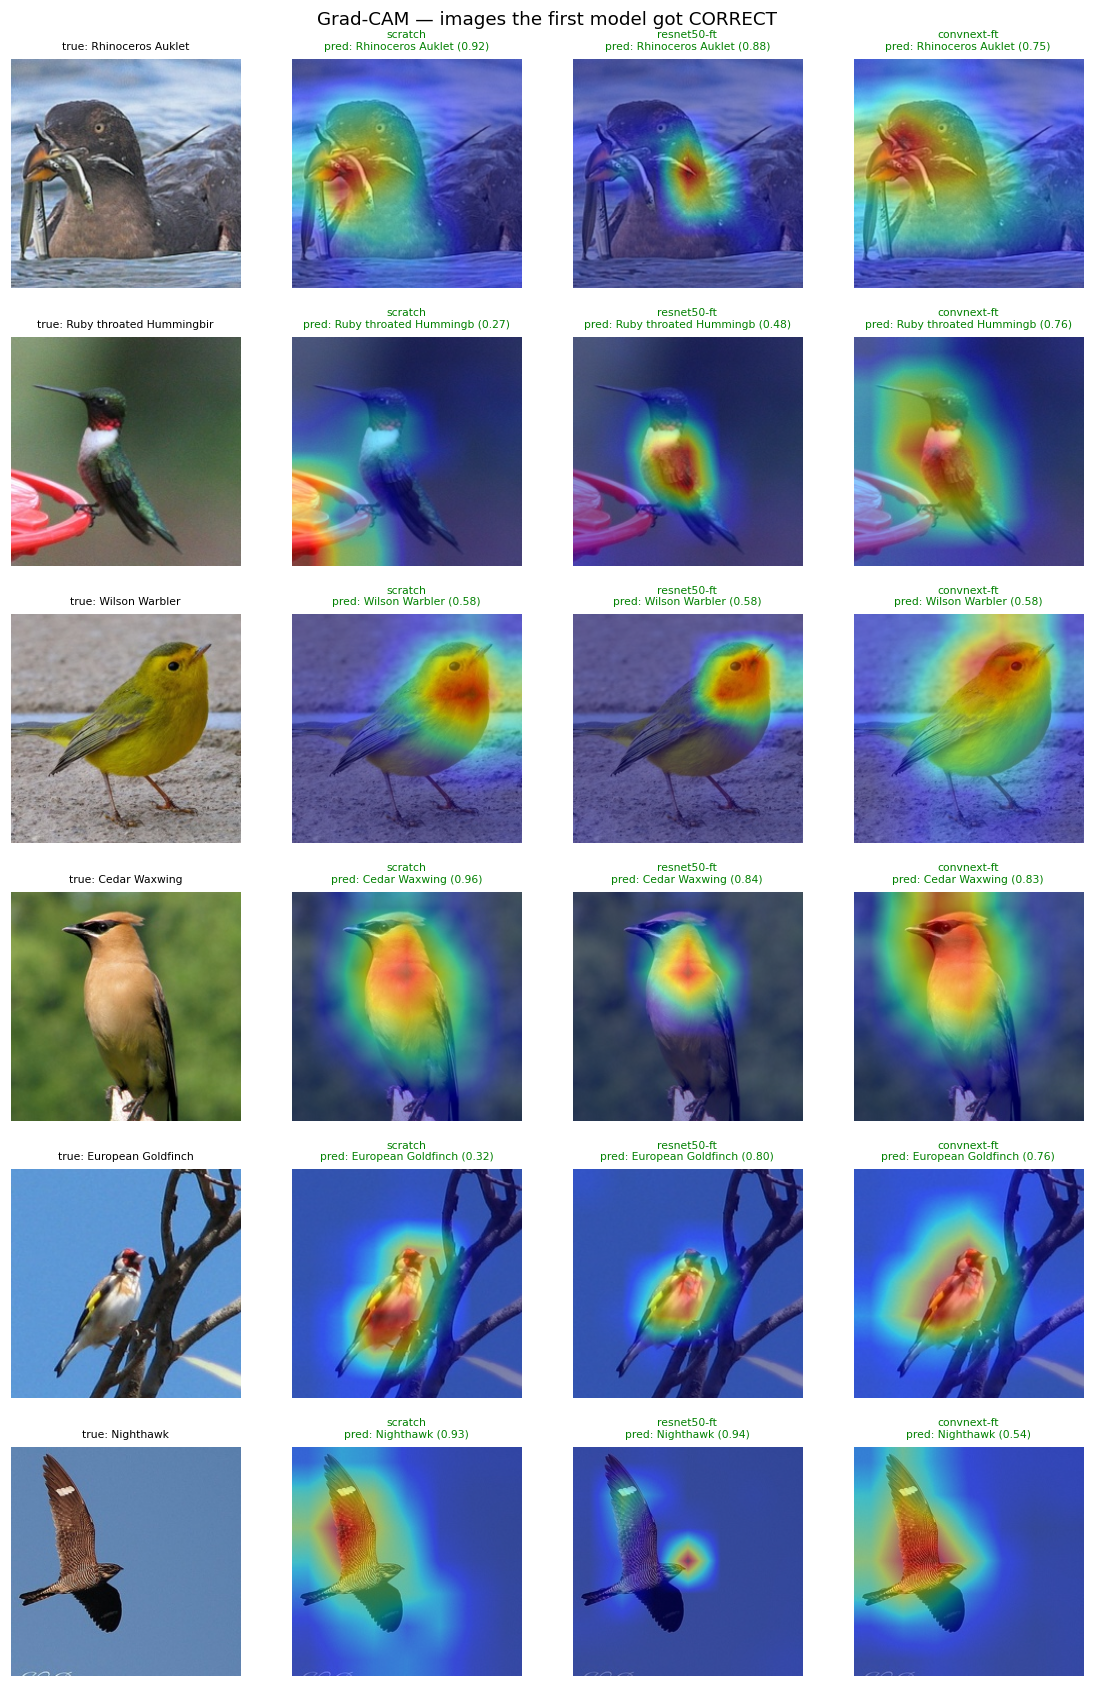
\includegraphics[width=0.8\linewidth]{figs/gradcam_correct.png}
\caption{Grad-CAM on images the scratch CNN classified correctly (green: correct, red: wrong; confidence in brackets).}\label{fig:gc1}
\end{figure}
\begin{figure}[H]\centering
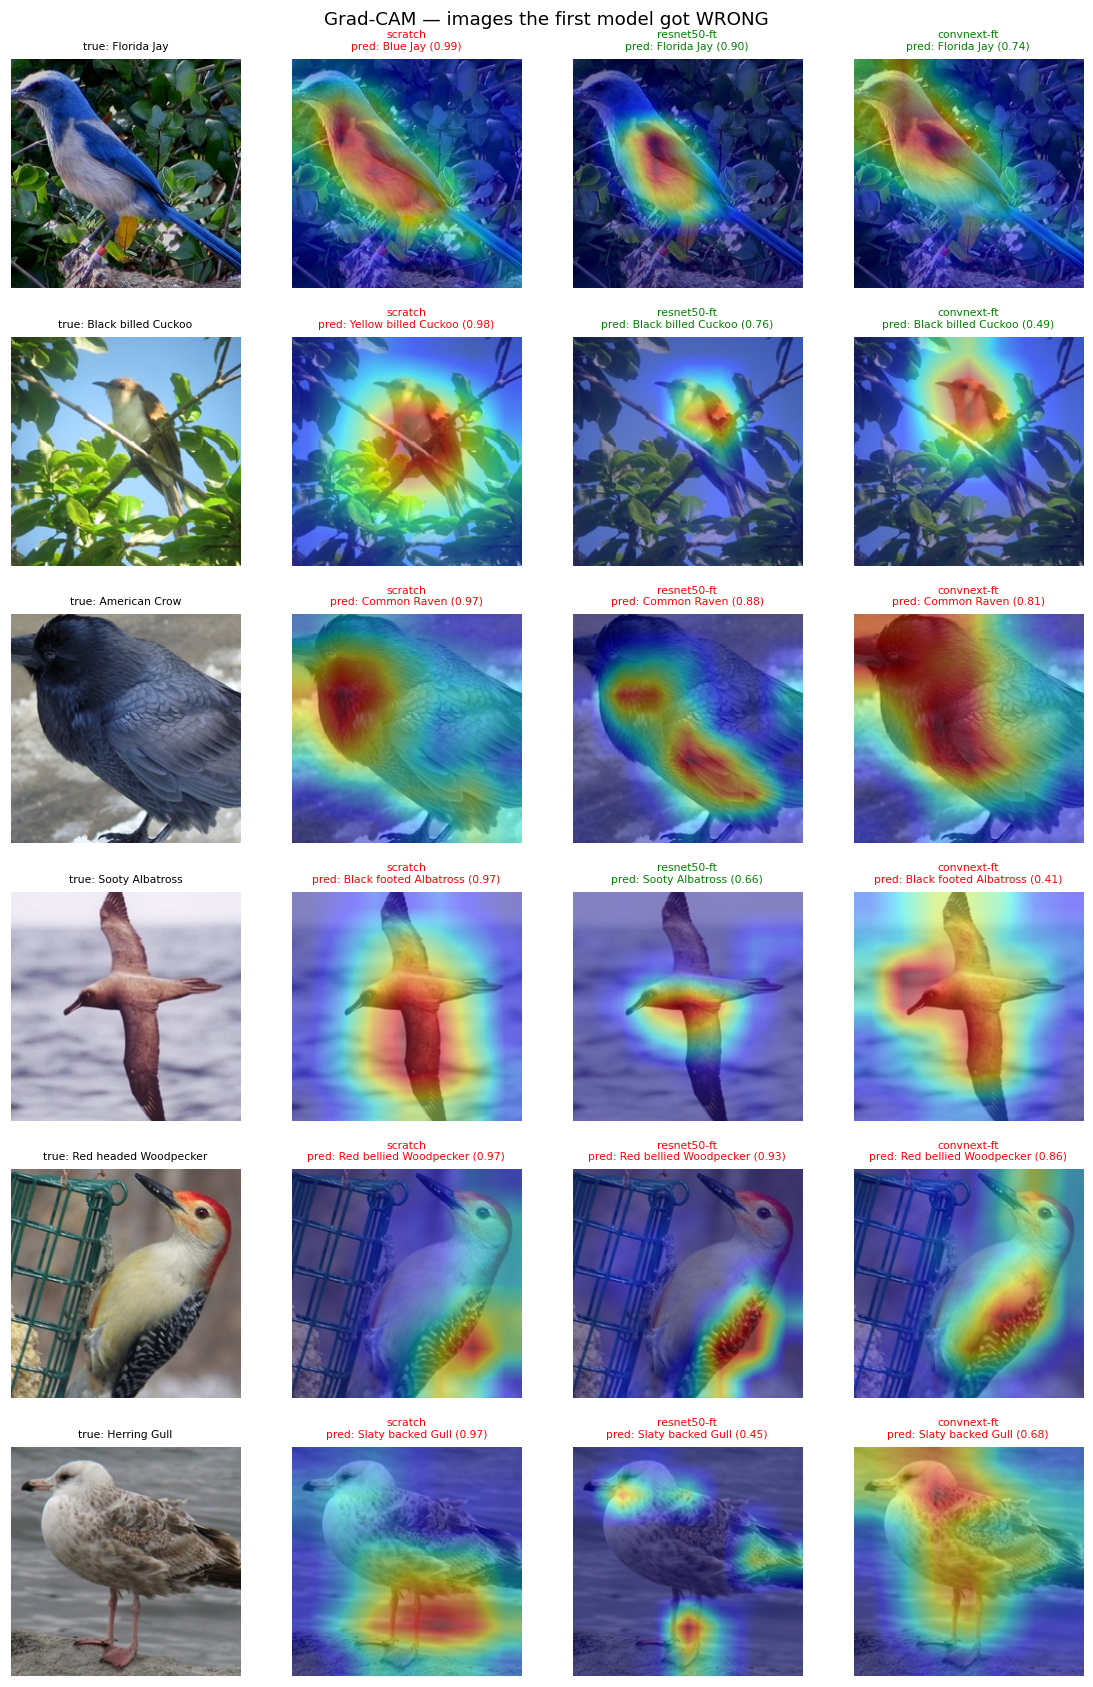
\includegraphics[width=0.8\linewidth]{figs/gradcam_wrong.png}
\caption{Grad-CAM on the scratch CNN's most confident mistakes.}\label{fig:gc2}
\end{figure}

\textbf{Analysis.}
\begin{itemize}
\item \textbf{Correct predictions} (Fig.~\ref{fig:gc1}): all models mostly look at the bird, typically the head and breast,
where most field marks are (e.g.\ the Wilson's Warbler's head, the Cedar Waxwing's face and crest).
The pretrained models produce tighter, part-focused maps (ResNet-50 on the hummingbird's red throat), while the scratch
CNN's maps are broader.
\item \textbf{Right for the wrong reason:} on the Ruby-throated Hummingbird the scratch CNN's attention is on the
\emph{red feeder}, not on the bird (and its confidence is only 0.27). It has learned a context shortcut --- red objects near
hummingbirds --- that will not generalise; the pretrained models attend to the bird itself.
\item \textbf{Scratch mistakes are confident and coarse} (Fig.~\ref{fig:gc2}): it predicts Blue Jay for a Florida Jay with 0.99
confidence while attending to the whole body; the fine-tuned models, attending to the same region but with better features,
get it right. For the Herring Gull the scratch CNN looks at the ground and legs.
\item \textbf{Mistakes shared by all models are informative:} American Crow $\rightarrow$ Common Raven is wrong for all three:
the two are separated mainly by size and bill thickness, which a single cropped image does not show reliably. The
Red-headed Woodpecker is predicted as Red-bellied Woodpecker by all models, whose attention lies on the barred back/belly
--- shared by both species --- rather than on the fully red head that distinguishes it.
\end{itemize}

%=====================================================================
\section{Benchmarking}\label{sec:bench}
%=====================================================================
We compare against published results on the same benchmark: the official CUB-200-2011 test split (5,794 images, which we did
not modify) and the same metric (top-1 accuracy). The open-source pretrained backbones are additionally evaluated by us on
our split with our metrics (Table~\ref{tab:results}).

\begin{table}[H]\centering\small
\begin{tabular}{llccc}
\toprule
Method & Backbone (pretraining) & Input & Top-1 (\%) & Source\\
\midrule
\multicolumn{5}{l}{\emph{Trained from scratch}}\\
ResNet-50, 300 epochs$^\dagger$ & ResNet-50 (none) & -- & 66.7 & \cite{featmining}\\
ResNet-50 + cross-entropy & ResNet-50 (none) & 448 & 51.9 & \cite{cosine}\\
ResNet-50 + cosine loss + cross-entropy & ResNet-50 (none) & 448 & 68.0 & \cite{cosine}\\
Ours, scratch CNN, 80 epochs (baseline) & 11M CNN (none) & 224 & 52.5 & \\
\textbf{Ours, scratch CNN, final}$^\ddagger$ & 11M CNN (none) & 224 & \textbf{66.8} & \\
\midrule
\multicolumn{5}{l}{\emph{Fine-tuned ImageNet backbones}}\\
ResNet-50 (+2 FC layers) & ResNet-50 (IN-1k) & 224 & 77.5 & \cite{posthoc}\\
ResNet-50 baseline & ResNet-50 (IN-1k) & 448 & 84.5 & \cite{nts}\\
ResNet-50 baseline & ResNet-50 (IN-1k) & 448 & 85.3 & \cite{cutthumb}\\
NTS-Net (part-based) & ResNet-50 (IN-1k) & 448 & 87.5 & \cite{nts}\\
TransFG (state of the art class) & ViT-B/16 (IN-21k) & 448 & 91.7 & \cite{transfg}\\
\textbf{Ours, ResNet-50 fine-tune} & ResNet-50 (IN-1k) & 224 & \textbf{82.4} & \\
Ours, ConvNeXt-Tiny fine-tune (baseline) & ConvNeXt-T (IN-1k) & 224 & 84.6 & \\
\textbf{Ours, ConvNeXt-Tiny final} & ConvNeXt-T (IN-1k) & 384 & \textbf{87.0} (87.3 TTA) & \\
\bottomrule
\end{tabular}
\caption{Comparison with published results on the CUB-200-2011 test split. $^\dagger$Reported by the authors as ``validation accuracy''. $^\ddagger$Uses ground-truth bird boxes at test time.}
\end{table}

\textbf{Discussion of the differences.}
\begin{itemize}
\item \textbf{Resolution} is the largest factor. Standard fine-grained baselines use $448\times448$ inputs; at 224\,px our
fine-tuned ResNet-50 (82.4\%) is about 2--3 points below the 448\,px ResNet-50 baselines (84.5--85.3\%), consistent
with small field marks being lost at lower resolution. At the same 224\,px resolution our ResNet-50 is well above the 77.5\%
reported in~\cite{posthoc}; part of this is our training recipe (AdamW, discriminative LRs, label smoothing, augmentation)
and the stronger torchvision ImageNet weights (\texttt{IMAGENET1K\_V2}) we start from.
\item \textbf{ConvNeXt-Tiny at 224\,px matches ResNet-50 at 448\,px} (84.6\% vs.\ 84.5\%) with about four times fewer input
pixels, showing the benefit of a newer architecture.
\item \textbf{Our final model} (87.0\%, full image, 384\,px, no annotations) is above the 448\,px ResNet-50 baselines
(84.5--85.3\%) and close to the part-based NTS-Net (87.5\%), with a standard architecture and no part-localisation module.
\item \textbf{From scratch, the cosine loss reproduces the published trend}: Barz \& Denzler~\cite{cosine} report 51.9\%
(cross-entropy) vs.\ 68.0\% (cosine + cross-entropy) for a ResNet-50 trained from scratch on CUB; our 11M-parameter CNN goes from
52.5\% to 66.8\% with the cosine loss, bird crops and Mixup/CutMix. Their numbers do not use bounding boxes, ours do, so this row is
a trend comparison rather than a like-for-like one.
\item \textbf{The gap to the state of the art} (TransFG, 91.7\%) comes from three things we do not use: a ViT-B/16 pretrained on the
$14\times$ larger ImageNet-21k, 448\,px input, and explicit part-selection mechanisms designed for fine-grained recognition.
\item \textbf{From scratch}, our baseline CNN was far below the 300-epoch ResNet-50 of~\cite{featmining} (52.5\% vs.\ 66.7\%); with
the improvements of Section~\ref{sec:improve} our final scratch CNN (66.8\%) matches it with half the parameters, but with bounding boxes.
\item \textbf{Limits of the comparison}: we report a single seed, while published baselines differ in epochs, optimisers and
augmentation; these numbers should be read as reference points, not as a controlled comparison.
\end{itemize}

%=====================================================================
\section{Improving the models}\label{sec:improve}
%=====================================================================
After the baseline experiments we tested a series of improvements, \textbf{one change at a time} so that
the effect of each can be measured. Ideas came from the EDA, from the Grad-CAM analysis, from the literature and
from team discussion. As before, \textbf{every choice is made on the validation set}; the test set is only
reported. All runs in this section use a higher-resolution image cache (shorter side 512\,px instead of 256\,px).
This alone changes results slightly: the standard ResNet-50 recipe re-run on the new cache scored 83.8\% instead of
82.4\% (sharper crops when RandomResizedCrop zooms in, plus run-to-run noise). We therefore compare
\emph{within} each series and always include a re-run baseline.

%---------------------------------------------------------------------
\subsection{Bird-crop preprocessing (bounding boxes)}
\textbf{Motivation.} The bird covers only \textbf{32\% of the image} on median (as little as 5\%; 2,739 images are under
20\%, Fig.~\ref{fig:birdcrop}), so about two-thirds of every input is background (branches, water, feeders). Grad-CAM had
already shown that the scratch CNN used the red feeder rather than the hummingbird --- a background shortcut.

\textbf{Method.} The Hugging Face version of CUB has no annotations, so we extracted the official bounding boxes
(\texttt{bounding\_boxes.txt}) from the original CUB-200-2011 release once and matched them to all 11,788 images by file name
(\texttt{resources/cub\_bounding\_boxes.csv}). Each image is cropped to a \emph{square} box around the bird with a 15\% margin on
every side (\texttt{crop\_to\_bird} in \texttt{src/data/datasets.py}), so that the later centre crop does not cut off tails or
wings, and some context remains. The crop is applied identically to train, validation and test images; all other preprocessing
and augmentation then run on the cropped image.

\begin{figure}[H]\centering
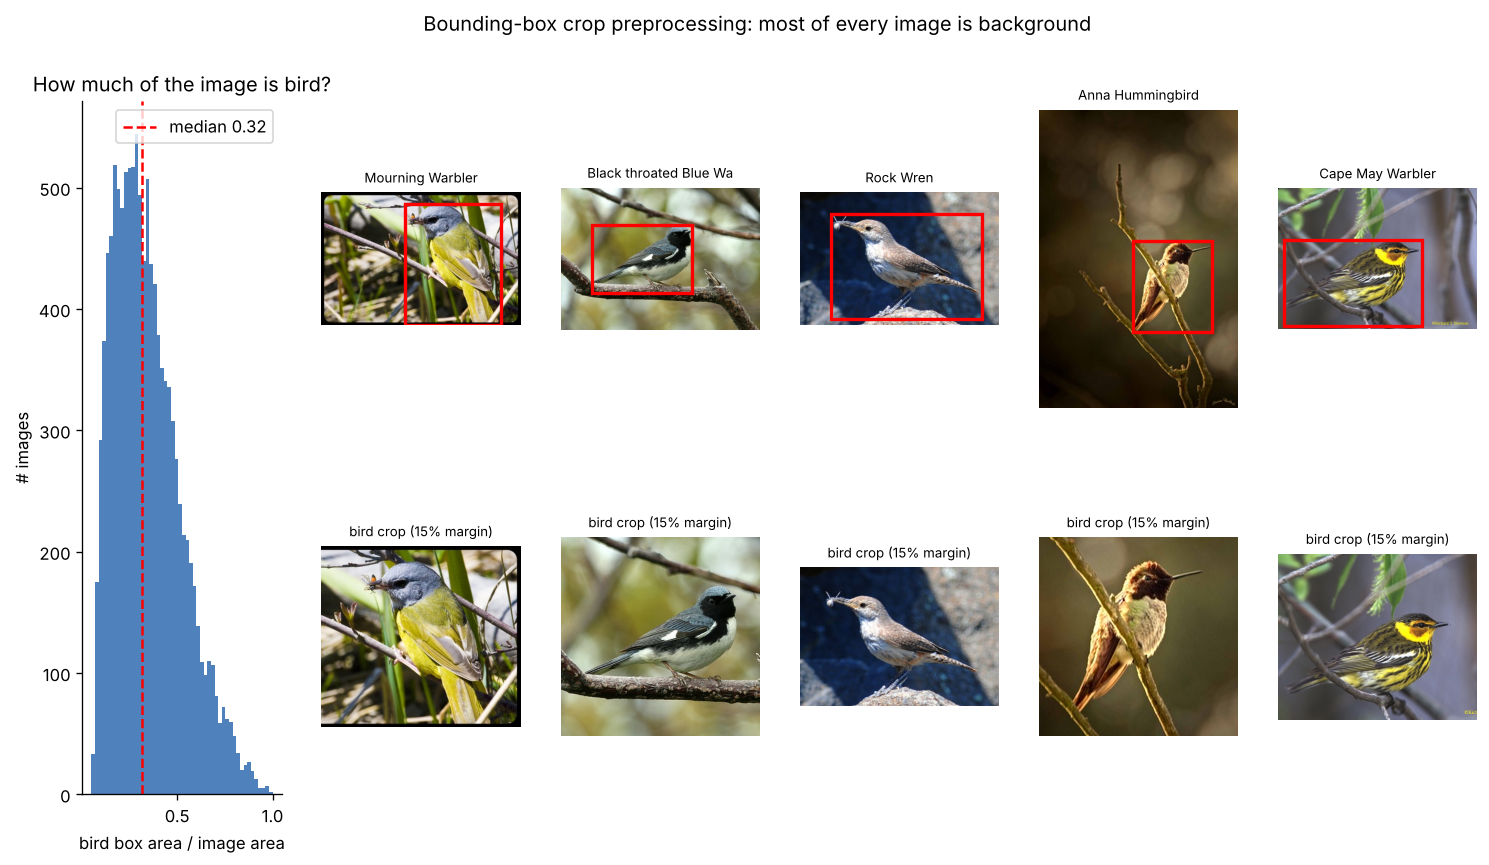
\includegraphics[width=\linewidth]{figs/14_bird_crop.png}
\caption{Left: fraction of the image covered by the bird. Right: original images with the official box (top) and our crop (bottom).}\label{fig:birdcrop}
\end{figure}

\textbf{Results.} Cropping is the single most effective change: \textbf{+6.3 points} for the scratch CNN (52.5\%$\rightarrow$58.7\%)
and \textbf{+1.3 points} for ConvNeXt-Tiny (84.6\%$\rightarrow$85.9\%). It helps the scratch CNN much more because a network that
learns from 5,400 images cannot afford to spend capacity on background, while ImageNet features already ignore much of it.
Cropping also acts as a \emph{zoom}: the bird occupies the whole $224\times224$ input, so field marks get about $3\times$ more pixels.

\textbf{Caveat (fairness).} Using the ground-truth box \emph{at test time} uses an annotation that a real user would not provide.
These results are therefore reported separately as ``with ground-truth boxes'' and are not compared with annotation-free methods;
we also report our best \emph{full-image} model. In a deployed system (and for Milestone~2) a bird detector would supply the box.

%---------------------------------------------------------------------
\subsection{Resolution}
At 384\,px (instead of 224) on full images, ConvNeXt reached a higher validation accuracy (85.1\% vs.\ 84.3\%) but the same test
accuracy (84.6\%); its best epoch came early (14 of 30) and it costs $2.3\times$ more time per epoch. With the bird crop, 384\,px
added +0.3 points (85.9\%$\rightarrow$86.2\%). \textbf{Conclusion:} at our budget, cropping is a cheaper and more effective
``zoom'' than raising the resolution of the whole image; the two partly do the same thing.

%---------------------------------------------------------------------
\subsection{Augmentation ablation}
Seven augmentation strategies were compared on the same model (ResNet-50 fine-tune, full image, 224\,px, 30 epochs):

\begin{figure}[H]\centering
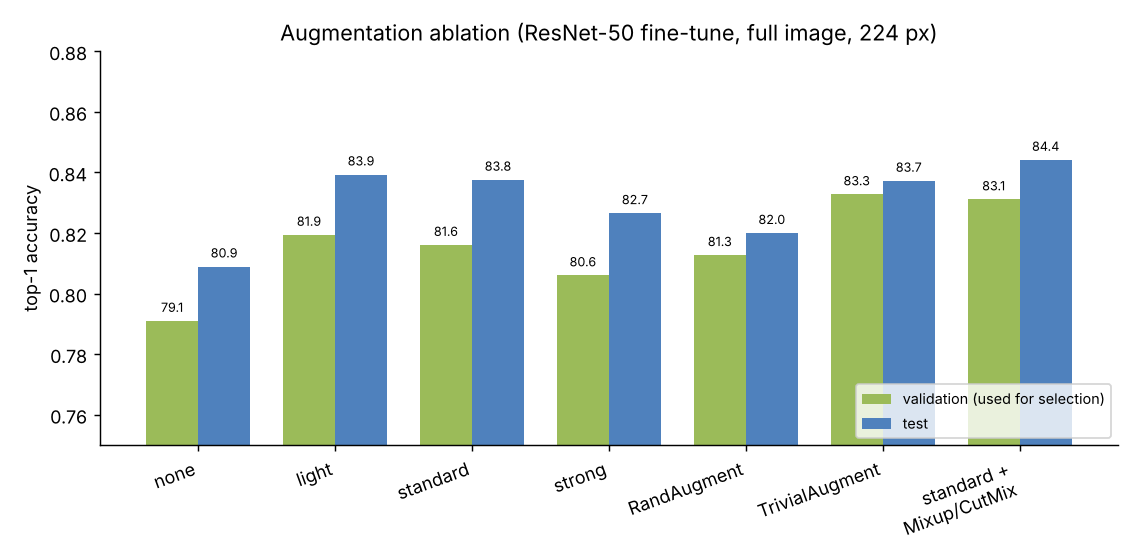
\includegraphics[width=0.85\linewidth]{figs/ablation_aug.png}
\caption{Augmentation ablation: validation (selection) and test accuracy.}\label{fig:augabl}
\end{figure}

\begin{itemize}
\item \textbf{Augmentation matters}: with none, test accuracy is 80.9\%; every geometric augmentation improves it by about 2--3 points.
\item \textbf{Light $\approx$ standard} (83.9\% vs.\ 83.8\%, within noise).
\item \textbf{Too strong hurts}: \emph{strong} (82.7\%) sometimes crops the bird out entirely (Fig.~\ref{fig:aug}).
\item \textbf{RandAugment is the worst augmented setting (82.0\%)}. Its policy includes colour-changing operations (Color, Solarize,
Posterize, Equalize). This supports our EDA-based decision not to alter colours: colour is a label-relevant feature for birds.
TrivialAugment, whose operations are sampled with random strength (often weak), stays at the standard level (83.7\%).
\item \textbf{Mixup/CutMix on top of standard is the best} (84.4\% test, 85.0\% with TTA). Mixup blends two images and their labels;
CutMix pastes a patch of one image into another and mixes the labels by area. Both prevent the model from becoming over-confident on
27 images per class. (The low ``train accuracy'' of mixed runs, $\sim$67\%, is measured on the mixed images and is expected.)
\end{itemize}

%---------------------------------------------------------------------
\subsection{Loss function: cosine loss vs.\ cross-entropy}
Cross-entropy keeps pushing the true-class logit up, so on a tiny dataset the network can reduce the loss simply by
\emph{scaling up} its outputs. The cosine loss of Barz \& Denzler~\cite{cosine}, proposed for small datasets trained from scratch,
L2-normalises the output vector and maximises its cosine similarity with the one-hot vector of the true class, so only the
\emph{direction} of the output matters. We implemented their combined form, cosine loss $+\,0.1\times$ cross-entropy on the
normalised vector (\texttt{src/training/losses.py}); predictions use the (scaled) cosine similarities.

\begin{figure}[H]\centering
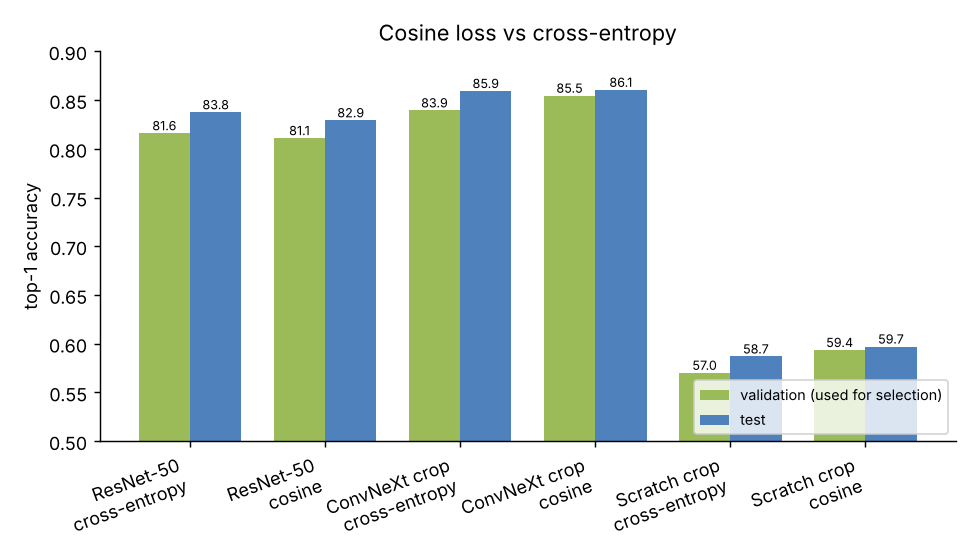
\includegraphics[width=0.85\linewidth]{figs/loss_compare.png}
\caption{Cosine loss vs.\ cross-entropy for three models.}\label{fig:loss}
\end{figure}

\textbf{Results.} As the paper predicts, the cosine loss helps most when training \textbf{from scratch} (+1.0 test, +2.3 validation).
For the pretrained ConvNeXt it improved validation accuracy by 1.5 points (the best single-change validation score, 85.5\%) but test
accuracy only by 0.1; for ResNet-50 it was 0.8 points \emph{worse} on test. With pretrained features the over-confidence problem the
cosine loss addresses is smaller, so its benefit is inconsistent.

%---------------------------------------------------------------------
\subsection{Scratch CNN: combining the improvements}
\begin{figure}[H]\centering
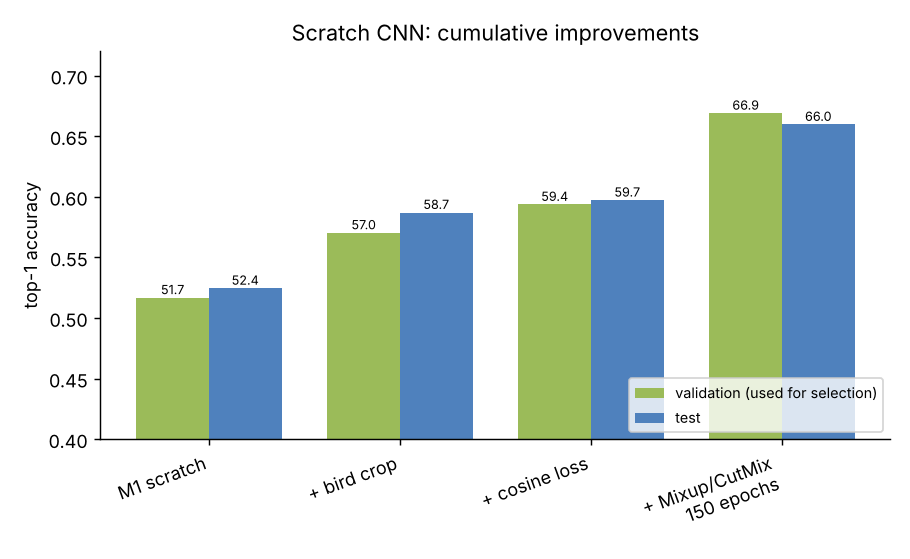
\includegraphics[width=0.7\linewidth]{figs/improve_scratch.png}
\caption{Cumulative improvements of our from-scratch CNN.}
\end{figure}
Bird crop (+6.3), cosine loss (+1.0), then Mixup/CutMix with longer training (150 epochs, +6.2) raised the scratch CNN from
52.5\% to \textbf{66.0\%} (66.6\% with TTA), a gain of 13.5 points without any pretraining. The overfitting gap also shrank: the original
model reached 96\% training accuracy against 51\% validation; with mixing the model can no longer memorise individual images.
Validation accuracy was still rising at epoch 147 of 150, so a longer run is included in the final experiments.

%---------------------------------------------------------------------
\subsection{Test-time augmentation (TTA)}
At test time each image is also classified mirrored (horizontal flip) and the two probability vectors are averaged. TTA improved
\textbf{all 16 runs}, by +0.58 points on average (range +0.22 to +1.07), at the cost of a second forward pass. Being free of training,
it is reported for every run from now on.

%---------------------------------------------------------------------
\subsection{Hyper-parameter tuning v2}
Tuning v1 had one clear limitation: the 8-epoch proxy runs favoured fast-converging settings, and the tuned configuration did not beat
the default at 30 epochs. Tuning v2 fixes the protocol: (i) a 15-epoch proxy, (ii) on the final model family (ConvNeXt-T + bird crop)
rather than ResNet-50, and (iii) four hyper-parameters --- head LR, \textbf{backbone LR multiplier}, weight decay, label smoothing ---
with random search (8 trials).

\begin{figure}[H]\centering
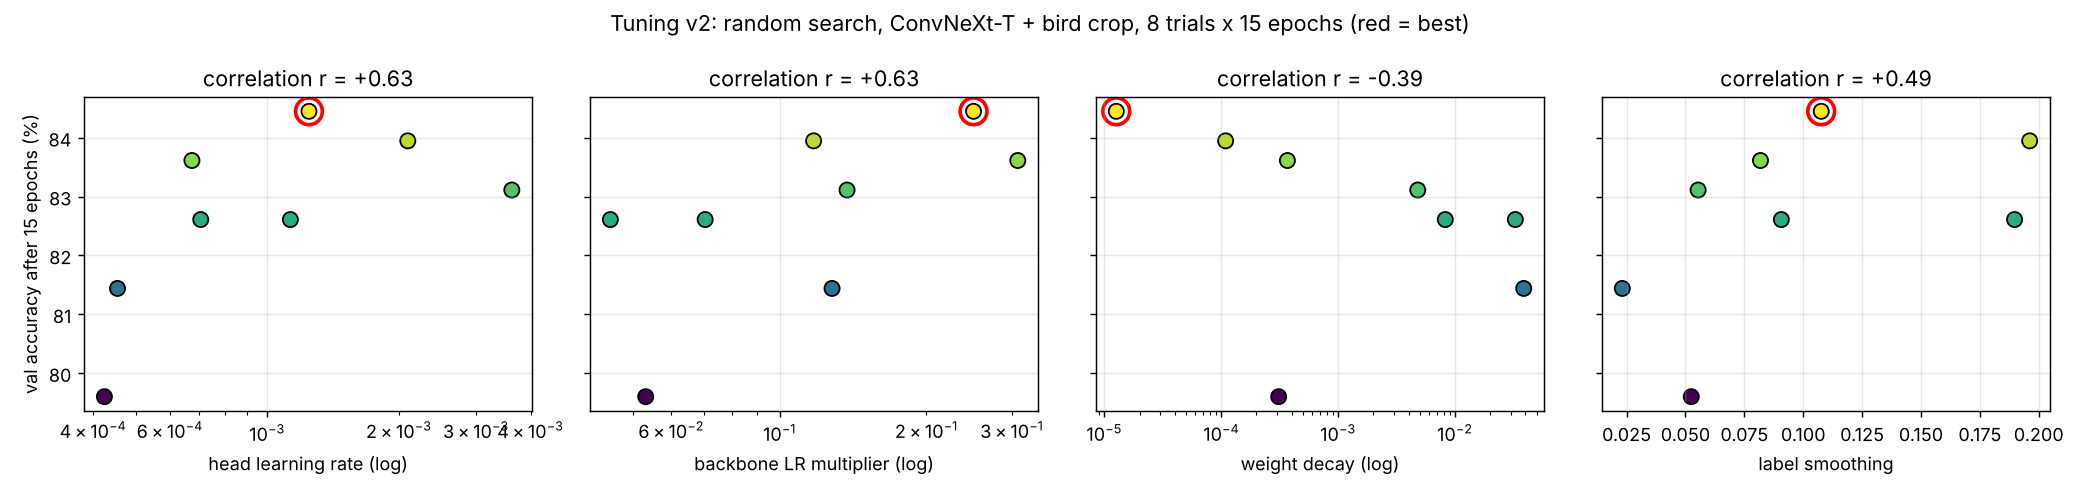
\includegraphics[width=\linewidth]{figs/tuning_v2_params.png}
\caption{Tuning v2: validation accuracy of each trial against each hyper-parameter (red circle = best trial).}\label{fig:tunev2}
\end{figure}

The best trial reached 84.5\% validation accuracy after only 15 epochs (head LR $1.25\!\times\!10^{-3}$, backbone multiplier 0.25,
weight decay $1.3\!\times\!10^{-5}$, label smoothing 0.11). The new parameter was informative: validation accuracy correlates positively
with the \textbf{backbone LR multiplier} ($r=+0.63$) --- trials with a multiplier around 0.05--0.07 were among the worst. Our default of 0.1
adapts the backbone too gently for fine-grained birds; a larger multiplier lets the deeper layers learn bird-specific features. With
eight trials these correlations are indicative only. The tuned values are used in the final combined runs.

%---------------------------------------------------------------------
\subsection{Summary of single changes (ConvNeXt-Tiny)}
\begin{figure}[H]\centering
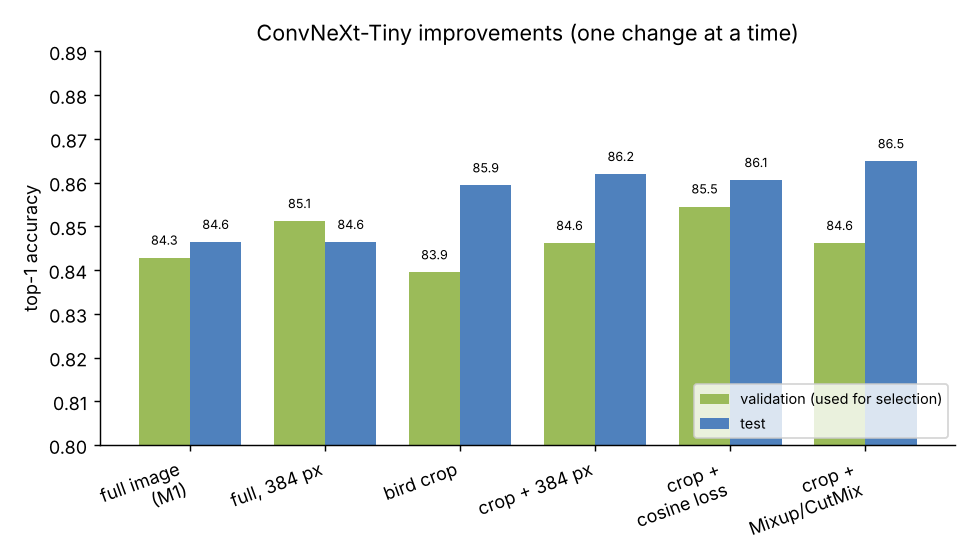
\includegraphics[width=0.85\linewidth]{figs/improve_convnext.png}
\caption{ConvNeXt-Tiny: one change at a time (validation and test accuracy).}
\end{figure}

\begin{table}[H]\centering\small
\begin{tabular}{lcccc}
\toprule
ConvNeXt-Tiny run & Val & Test & Test + TTA & Macro-F1\\
\midrule
Full image, 224\,px (Milestone-1 baseline) & 84.3 & 84.6 & --- & 84.5\\
Full image, 384\,px & 85.1 & 84.6 & 84.9 & 84.5\\
Bird crop, 224\,px & 83.9 & 85.9 & 86.3 & 85.8\\
Bird crop, 384\,px & 84.6 & 86.2 & 86.5 & 86.1\\
Bird crop, cosine loss & \textbf{85.5} & 86.1 & 86.5 & 86.0\\
Bird crop, Mixup/CutMix (40 ep.) & 84.6 & \textbf{86.5} & \textbf{86.7} & \textbf{86.4}\\
\bottomrule
\end{tabular}
\caption{ConvNeXt-Tiny improvements (\%). Validation differences below $\sim$1.5 points are within noise (598 images).}
\end{table}

%FINALRUNS


%=====================================================================
\section{Final selection}
%=====================================================================
\textbf{Classifier: ConvNeXt-Tiny, fully fine-tuned on full images at 384\,px with Mixup/CutMix and the tuning-v2 hyper-parameters}
(\texttt{configs/improve/final\_full\_ce.yaml}). It has the best validation accuracy of all runs (87.3\% --- this is how it was
\emph{selected}; the test set was only used for reporting) and reaches \textbf{87.0\% test accuracy, 87.3\% with flip TTA}, 87.2\%
macro-F1 and 97.1\% top-5. It needs no bounding box at inference. Training takes 55 minutes on a T4. \textbf{Best from-scratch model:}
our residual CNN with bird crops, cosine loss and Mixup/CutMix, 250 epochs: 66.8\% (67.5\% with TTA).

\textbf{Encoder for Milestone 2.} The final fine-tuned ConvNeXt-Tiny encoder will be the main backbone for colorization and captioning:
it provides the best bird-specific features and four feature maps (96--768 channels, strides 4--32) that plug directly into a
U-Net decoder. Fine-tuned ResNet-50 is kept as a second backbone for comparison, and the scratch CNN as the from-scratch baseline.
All three checkpoints are stored in the shared Google Drive folder.

%=====================================================================
\section{Failures and limitations}\label{sec:fail}
%=====================================================================
\begin{itemize}
\item \textbf{Scratch CNN overfitting.} The baseline overfit strongly (96\% train vs.\ 51\% validation). Bird crops, the cosine
loss, Mixup/CutMix and longer training raised it to 66.8\%, but Grad-CAM shows it still relies on background context.
\item \textbf{The CNN without residual connections failed to train well} (44\% training accuracy): this was an intended
ablation, but it confirms that plain 18-layer CNNs are hard to optimise.
\item \textbf{Tuning v1 did not transfer to the full schedule}: the 8-epoch optimum gave no improvement at 30 epochs. Tuning v2
(15-epoch proxy, 4 hyper-parameters, final model family) produced the settings used by the final model. Still open: several seeds,
Optuna/Hyperband, and tuning augmentation strength.
\item \textbf{Some ideas did not work}: RandAugment and the \emph{strong} augmentation \emph{lowered} accuracy; 384\,px on full
images gave no test gain on its own; the cosine loss was worse than cross-entropy for ResNet-50.
\item \textbf{Ground-truth boxes}: the crop experiments use annotations that are not available for new photos; the final model
therefore does not use them. A bird detector would be needed to use cropping in practice.
\item \textbf{Label noise}: at least 4\% of CUB labels are estimated to be wrong~\cite{vanhorn}; several confident ``errors'' of our
final model look like such cases.
\item \textbf{Single seed and a small validation set} (598 images): differences below $\sim$1.5 points are not statistically reliable.
\item \textbf{Resolution}: baseline runs used 224\,px; the final model uses 384\,px. 448\,px and larger backbones
(ConvNeXt-Small/Base, ImageNet-21k weights) were not tried because of the GPU budget.
\item \textbf{Infrastructure}: the first Kaggle runs silently ran without GPU or internet because the account was not phone-verified;
our CLI now refuses to train on a CPU unless explicitly allowed, and the code, data and weights are packaged so the jobs can run
offline.
\item \textbf{Label noise} (e.g.\ the nightjar pair) and genuinely ambiguous pairs (crow/raven) cap achievable accuracy.
\end{itemize}

%=====================================================================
\section{Reproducibility and interface}
%=====================================================================
All final code is pure Python, run through the CLI (\texttt{src/cli.py}); notebooks are not used for the final code. Exact commands:
{\footnotesize
\begin{verbatim}
python -m src.cli doctor          # checks GPU, CUDA PyTorch, W&B login, data
python -m src.cli prepare         # download, cache, split, deduplicate
python -m src.cli eda
python -m src.cli prepare --out data/processed_hr --short-side 512     # high-resolution cache
python -m src.cli train --task classification --config configs/improve/final_full_ce.yaml
python -m src.cli tune  --config configs/tune_resnet50.yaml --method grid    # or random
python -m src.cli compare-tuning --dirs outputs/tuning/grid_* outputs/tuning/random_*
python -m src.cli evaluate --task classification --checkpoint <run>/best.pt --split test
python -m src.cli predict  --task classification --checkpoint <run>/best.pt --image bird.jpg
python -m src.cli gradcam  --checkpoints <scratch>/best.pt <resnet50>/best.pt --names scratch resnet50
python -m src.cli compare  --runs outputs/runs/*
\end{verbatim}
}
Seeds are fixed, the validation split is stored in \texttt{data/processed/metadata.csv}, and every run folder and checkpoint
contains the exact configuration it was trained with.

%=====================================================================
\section{Team contributions}
%=====================================================================
\begin{table}[H]\centering\small
\begin{tabular}{p{4.2cm}p{11cm}}
\toprule
Member & Contribution\\
\midrule
Abdelrahman Mohamed Zayed & Repository and project structure, data pipeline, EDA, training/tuning pipeline, improvement experiments (bird crop, cosine loss, Mixup/CutMix, TTA, tuning v2), Kaggle and W\&B setup, report\\
Yehya ElAbyad & Data module: tests for caption cleaning, tokenizer, vocabulary, transforms and dataset; data pipeline documentation (PR \#3)\\
Ahmed ElSayed & Models: encoder and classifier contract tests (incl.\ cosine head and checkpoints), CPU encoder summary script, architecture documentation (PR \#2)\\
Saeed Mohamed Negm & Training: config, scheduler/optimizer and tuning tests, training documentation\\
Hassan Hazem & Evaluation: metric and Grad-CAM tests, batch (folder) inference feature, evaluation documentation (PR \#1)\\
\bottomrule
\end{tabular}
\end{table}

%=====================================================================
\begin{thebibliography}{99}\small
\bibitem{cub} C.~Wah, S.~Branson, P.~Welinder, P.~Perona, S.~Belongie. \emph{The Caltech-UCSD Birds-200-2011 Dataset}. Caltech Tech.\ Report CNS-TR-2011-001, 2011.
\bibitem{reed} S.~Reed, Z.~Akata, H.~Lee, B.~Schiele. Learning Deep Representations of Fine-Grained Visual Descriptions. CVPR 2016.
\bibitem{resnet} K.~He, X.~Zhang, S.~Ren, J.~Sun. Deep Residual Learning for Image Recognition. CVPR 2016.
\bibitem{effnet} M.~Tan, Q.~Le. EfficientNet: Rethinking Model Scaling for Convolutional Neural Networks. ICML 2019.
\bibitem{convnext} Z.~Liu, H.~Mao, C.-Y.~Wu, C.~Feichtenhofer, T.~Darrell, S.~Xie. A ConvNet for the 2020s. CVPR 2022.
\bibitem{gradcam} R.~R.~Selvaraju et al. Grad-CAM: Visual Explanations from Deep Networks via Gradient-based Localization. ICCV 2017.
\bibitem{bergstra} J.~Bergstra, Y.~Bengio. Random Search for Hyper-Parameter Optimization. JMLR 13, 2012.
\bibitem{kornblith} S.~Kornblith, J.~Shlens, Q.~V.~Le. Do Better ImageNet Models Transfer Better? CVPR 2019.
\bibitem{nts} Z.~Yang et al. Learning to Navigate for Fine-grained Classification (NTS-Net). ECCV 2018. \url{https://arxiv.org/abs/1809.00287}
\bibitem{cutthumb} Cut-Thumbnail: A Novel Data Augmentation for Convolutional Neural Network. ACM MM 2021. \url{https://arxiv.org/abs/2103.05342}
\bibitem{posthoc} T.~Leemann et al. When are Post-hoc Conceptual Explanations Identifiable? UAI 2023. \url{https://arxiv.org/abs/2206.13872}
\bibitem{featmining} Feature Mining: A Novel Training Strategy for Convolutional Neural Network. \url{https://arxiv.org/abs/2107.08421}
\bibitem{transfg} J.~He et al. TransFG: A Transformer Architecture for Fine-grained Recognition. AAAI 2022. \url{https://arxiv.org/abs/2103.07976}
\bibitem{cosine} B.~Barz, J.~Denzler. Deep Learning on Small Datasets without Pre-Training using Cosine Loss. WACV 2020. \url{https://arxiv.org/abs/1901.09054}
\bibitem{mixup} H.~Zhang, M.~Cisse, Y.~N.~Dauphin, D.~Lopez-Paz. mixup: Beyond Empirical Risk Minimization. ICLR 2018.
\bibitem{cutmix} S.~Yun et al. CutMix: Regularization Strategy to Train Strong Classifiers with Localizable Features. ICCV 2019.
\bibitem{randaugment} E.~D.~Cubuk, B.~Zoph, J.~Shlens, Q.~V.~Le. RandAugment: Practical Automated Data Augmentation with a Reduced Search Space. CVPR Workshops 2020.
\bibitem{trivialaugment} S.~G.~M\"uller, F.~Hutter. TrivialAugment: Tuning-free Yet State-of-the-Art Data Augmentation. ICCV 2021.
\bibitem{vanhorn} G.~Van Horn et al. Building a Bird Recognition App and Large Scale Dataset with Citizen Scientists: The Fine Print in Fine-Grained Dataset Collection. CVPR 2015.
\bibitem{wandb} L.~Biewald. Experiment Tracking with Weights and Biases, 2020. \url{https://wandb.ai}
\bibitem{torchvision} TorchVision maintainers. TorchVision: PyTorch's Computer Vision library. \url{https://github.com/pytorch/vision}
\end{thebibliography}

\end{document}
